\documentclass[preprint,12pt]{elsarticle}

\usepackage{amsmath,amssymb}
\usepackage{booktabs}
\usepackage{multirow}
\usepackage{array}
\usepackage{graphicx}
\usepackage{adjustbox}
\usepackage{xcolor}
\usepackage{url}
\usepackage{hyperref}
\usepackage{longtable}

\journal{Engineering Applications of Artificial Intelligence}

\newcommand{\method}{VK-RMD}
\newcommand{\mpjpe}{MPJPE}
\newcommand{\pampjpe}{PA-MPJPE}

\begin{document}

\begin{frontmatter}

% Title selected for the EAAI-oriented manuscript:
% VK-RMD: Visual-Keypoint Anchored Missing-Modality Learning for Reduced-Visual-Exposure Multimodal Human Perception

\title{\method: Visual-Keypoint Anchored Missing-Modality Learning for Reduced-Visual-Exposure Multimodal Human Perception}

\author[1]{Author Name}
\address[1]{School of Computer Science and Technology, Dalian University of Technology, Dalian, China}

\begin{abstract}
Multimodal human perception is increasingly expected to operate in environments where raw RGB streams are undesirable at inference time and where sensing modalities may be intermittently unavailable. Existing multimodal human pose estimation (HPE) and human activity recognition (HAR) systems often rely on fixed input configurations; once depth, LiDAR, mmWave, WiFi-CSI, or visual-keypoint streams are missing or degraded, performance can collapse even when the full-modality model is accurate. This paper presents \method, a visual-keypoint (VK) anchored missing-modality learning framework for reduced-visual-exposure multimodal human perception. The central idea is to use VK as an appearance-suppressed structural bridge: RGB-derived visual knowledge is compressed into joint-level body geometry during training, while the deployable student performs inference from VK/non-RGB or fully non-visual modalities. Heterogeneous sensors are not forced into a shared raw space; instead, modality-specific encoders and projectors align them in a shared body-token space. The student is trained with random modality-subset sampling and a learned reliability proxy that dynamically weights available modalities under each missing pattern. Teacher-student supervision is used as an auxiliary training signal rather than the sole source of improvement. On MMFi-based HPE evaluation, \method{} Student-VK achieves 75.18 mm average \mpjpe{} over 31 modality combinations, compared with 103.70 mm for the official X-Fi/VK table baseline; the non-visual Student-NV achieves 84.68 mm over 15 non-visual combinations. On HAR, Student-VK achieves 85.15\% average accuracy over 15 combinations, compared with 62.46\% for the official/reproduced X-Fi/VK baseline, while Student-NV achieves 80.62\% over non-visual combinations. Fair internal baselines show that the method improves over uniform fusion in both tasks, while the HPE no-distillation result is competitive and therefore motivates a cautious, task-dependent interpretation of distillation. Cross-scene protocols expose remaining scene-shift limitations, which we report as an engineering boundary rather than hiding them.
\end{abstract}

\begin{keyword}
Multimodal human perception \sep missing modalities \sep visual keypoints \sep human pose estimation \sep human activity recognition \sep reliability-aware fusion \sep reduced visual exposure \sep non-RGB sensing
\end{keyword}

\end{frontmatter}

\begin{highlights}
\item A reduced-visual-exposure multimodal human perception framework is proposed.
\item VK acts as a structural bridge between RGB-derived knowledge and non-RGB sensing.
\item Random modality-subset training supports arbitrary modality combinations.
\item A learned reliability proxy improves fusion over uniform weighting under missing modalities.
\item HPE, HAR, cross-scene, cross-subject, and fair ablation results are reported.
\end{highlights}

\section{Introduction}

Human pose estimation (HPE) and human activity recognition (HAR) are two complementary tasks in human-centered artificial intelligence. HPE estimates fine-grained body geometry, typically through 2D or 3D joint coordinates; HAR recognizes action semantics, such as sitting, walking, or interacting with an environment. Many practical systems need both capabilities: geometry is needed to understand posture and body structure, while activity labels summarize the semantic state of a human subject. The engineering challenge is not merely to achieve high accuracy under complete laboratory inputs. A robust system must continue to function when some sensing channels are absent, noisy, or unsuitable for privacy-sensitive inference.

Raw RGB images are highly informative, but they are also privacy-sensitive. They expose identity cues, clothing, body appearance, and background context. In many long-term monitoring or human-computer interaction settings, continuous RGB inference is difficult to justify. Non-RGB modalities such as depth, LiDAR, mmWave radar, and WiFi channel state information (WiFi-CSI) provide alternatives with reduced visual exposure. However, these modalities are heterogeneous and noisy: depth can be affected by range and occlusion, LiDAR point clouds may be sparse for human bodies, mmWave radar can be noisy and variable, and WiFi-CSI is indirect and environment-dependent. A model that simply concatenates all available sensors and assumes a fixed modality set is therefore fragile.

Visual keypoints (VKs) provide a useful intermediate representation. They retain explicit human-body structure while suppressing most raw appearance and background information. Prior X-Fi/VK-style work shows that replacing raw RGB with structured keypoint representations can reduce visual exposure and preserve pose-related information. Nevertheless, using VKs alone does not solve arbitrary missing-modality robustness. A VK stream may itself be unavailable or inaccurate, and practical multimodal perception must work with variable subsets of non-RGB sensors. This motivates a broader formulation: reduced-visual-exposure multimodal human perception under missing modalities.

This paper proposes \method, a VK-anchored missing-modality learning framework. The method treats RGB as training-time privileged knowledge rather than an inference input. VKs act as a structural bridge from visual knowledge to deployable multimodal sensing: RGB is first compressed into an appearance-suppressed joint representation, and all available sensors are then projected into a shared body-token space. The student model is trained by randomly sampling modality subsets and by learning from ground-truth labels with optional full-modality teacher supervision. During inference, the student receives whatever modalities are available and uses a learned reliability proxy to dynamically assign weights to modality-specific evidence.

The paper follows an engineering application perspective. We do not claim to introduce knowledge distillation, skeleton representations, attention weighting, or modality dropout as isolated inventions. Instead, we focus on an integrated, testable solution to a practical problem: how to build a reduced-visual-exposure multimodal HPE/HAR model that does not require raw RGB at inference and remains usable under arbitrary modality combinations. The contribution is the formulation and validation of VK-anchored subset-invariant learning, rather than a claim that each individual component is new.

This distinction is important for the target venue. Engineering Applications of Artificial Intelligence papers are expected to connect an artificial-intelligence method to a real engineering need, to show why the design choices matter, and to demonstrate the method under realistic conditions. In this manuscript, the engineering need is robust human perception when privacy and sensor availability constraints prevent the use of a fixed RGB-centered pipeline. The artificial-intelligence component is not a single isolated module; it is a training and fusion strategy that combines VK-based structural supervision, missing-modality sampling, teacher-student learning, and reliability-aware decision weighting. The experimental evidence is therefore organized around application questions: Does the method work when all modalities are present? Does it remain usable when modalities are removed? Does it still work without VK? Does it generalize across scenes and subjects? Which component contributes most consistently?

The answer to these questions is mixed in a scientifically useful way. The proposed student improves average all-combination robustness over official/reproduced X-Fi/VK baselines in both HPE and HAR. Reliability-aware fusion is consistently better than uniform fusion, especially for HAR. Non-visual variants remain strong in full non-visual inference and acceptable in averaged missing-modality tests. At the same time, not every module is treated as a primary source of improvement. HPE no-distillation is competitive, showing that distillation is not the sole source of improvement. The exploratory Super-Teacher is not strong enough under missing combinations to be a main contribution. These boundaries are explicitly stated because a credible engineering paper reports both the effective design decisions and the limitations that matter for deployment.

The main contributions are:

\begin{itemize}
    \item We formulate VKs as an appearance-suppressed structural bridge between RGB-derived training knowledge and deployable multimodal inference, distinguishing our setting from direct raw-RGB inference and from simple fixed-modality fusion.
    \item We align heterogeneous sensors through a shared body-token space and train the student under randomly sampled modality subsets, so each available subset is treated as a valid sensing configuration.
    \item We use reliability-aware fusion as a learned modality-contribution proxy for dynamically weighting available modalities under each missing pattern.
    \item We validate the same framework on HPE and HAR, covering random, cross-scene, cross-subject, VK-enabled, and non-visual settings.
    \item We provide fair baseline, ablation, complexity, robustness, reliability-weight, and subset-level analyses, while clearly separating official/reproduced X-Fi/VK baselines and exploratory Super-Teacher results from our own main method.
\end{itemize}

\section{Related work}

\subsection{Reduced-exposure human sensing and visual keypoints}

RGB-based human perception has been widely studied because images provide dense visual cues. However, RGB inputs are often undesirable in privacy-sensitive human sensing. Visual keypoints and skeletons are commonly used as reduced representations of human structure. They preserve joint-level geometry while suppressing identity, clothing, and background appearance. This reduction is not a formal privacy guarantee, but it lowers visual exposure compared with raw images.

The X-Fi/VK line of work is particularly relevant because it motivates the use of structured visual representations in multimodal human perception. In this paper, reproduced X-Fi/VK results are treated as baselines. We do not present X-Fi/VK itself as our contribution. Our contribution begins from the observation that a VK-based model still needs robustness to arbitrary missing modalities and dynamic sensor reliability.

Reduced-exposure human sensing can be approached from several directions. One direction removes RGB entirely and relies on RF, acoustic, inertial, depth, or point-cloud signals. This reduces visual exposure but may weaken pose precision or semantic recognition. A second direction keeps RGB during inference but applies blurring, anonymization, or representation learning; such methods can still be questioned because raw visual capture remains part of the pipeline. A third direction uses structured body representations such as skeletons or keypoints. The third direction is the most relevant to our work because it retains the geometry needed by HPE and HAR while avoiding direct raw-RGB inference. However, VK alone is not sufficient: keypoints may be missing, noisy, or unavailable, and a robust system still needs non-RGB alternatives.

The paper therefore uses a two-level reduced-exposure formulation. Student-VK uses VK together with non-RGB modalities and removes raw RGB. Student-NV removes VK as well and uses only non-visual modalities. Reporting both variants prevents an overconfident privacy claim. Student-VK demonstrates the benefit of VK as a structural bridge; Student-NV demonstrates the feasibility of a stricter non-visual inference setting. VK may still reveal body geometry, gait, and action cues, so the manuscript does not claim formal anonymity, differential privacy, or cryptographic protection.

\subsection{Multimodal HPE and HAR}

Multimodal HPE combines visual and non-visual signals to infer body joints. Multimodal HAR combines complementary sensing streams to classify actions. These tasks are often studied separately, yet they are naturally connected: pose estimates describe body structure, and action labels describe temporal or semantic behavior. A robust human perception model is useful for both tasks. In this work, HPE and HAR are not two unrelated stories; they are two validation layers for the same reduced-visual-exposure missing-modality framework.

The two tasks also stress different failure modes. HPE is sensitive to geometric errors and therefore exposes whether the model preserves body structure under missing modalities. HAR is sensitive to semantic separability and therefore exposes whether the fused representation captures action-level information. A method that performs well only on HAR may hide poor structural precision; a method that performs well only on HPE may not support practical activity understanding. By evaluating both tasks, the paper tests whether the same robustness mechanism can support fine-grained regression and categorical recognition.

This dual-task evaluation is not a claim of a general-purpose human perception model. The current work evaluates two representative tasks available in the project pipeline. It does not claim to address tracking, forecasting, segmentation, identification, or interaction reasoning. This boundary keeps the contribution precise.

\subsection{Missing-modality learning}

Missing-modality learning addresses situations where a model cannot assume that all inputs are available. Common approaches include modality dropout, feature reconstruction, modality hallucination, mixture-of-experts fusion, and adaptive gating. Our setting differs from simple training-time dropout because the evaluation explicitly reports all valid modality combinations. For HPE, five modalities produce 31 non-empty combinations; for HAR, four modalities produce 15 non-empty combinations. This all-combination evaluation forces the model to handle both mild and severe missing patterns.

The all-combination protocol is demanding but useful. A method can appear robust if it is evaluated only under one or two manually selected missing cases. In contrast, exhaustive combination evaluation reveals whether robustness is broad or concentrated in easy cases. In our results, full-modality performance is strong, moderate missing patterns are generally robust, and single-modality cases are still difficult. This shape of results is more informative than a single average number because it identifies where the method is ready and where additional work is needed.

For the EAAI audience, the missing-modality problem is an engineering reliability problem. Sensors may be unavailable due to hardware failure, occlusion, privacy policy, environmental interference, or cost constraints. Training and testing only the full-modality configuration would overestimate real-world utility. The proposed random subset training and all-combination evaluation directly address this reliability concern.

\subsection{Reliability-aware multimodal fusion}

Uniform fusion treats all modalities as equally informative. This assumption is rarely valid in heterogeneous sensing. Different modalities vary in quality across scenes, subjects, and missing patterns. Reliability-aware fusion estimates dynamic weights for available modalities and therefore provides a more flexible engineering mechanism. In \method, the reliability module outputs normalized weights over the available modality tokens. These weights are interpreted as a learned modality-contribution proxy rather than a calibrated physical measurement of sensor reliability. The exported reliability-weight CSVs are used in this manuscript to visualize how the learned fusion module reallocates decision weight under different missing-modality patterns.

Reliability modeling also improves interpretability at the engineering level. It does not make the neural network fully transparent, but it gives a mechanism for asking which modalities receive larger decision weight under different input subsets. This is valuable for diagnosing sensor failures and for explaining why a model may rely more on depth in one setting and more on mmWave or VK in another. In this manuscript, reliability evidence is supported by performance ablations, exported average reliability weights, and subset-level correlation analysis.

\subsection{Teacher-student distillation for robust perception}

Teacher-student distillation transfers supervision from a stronger or more complete model to a student that is smaller, more deployable, or trained under restricted inputs. In our formulation, the teacher can use full-modality and VK/RGB-derived knowledge during training, while the final student is evaluated without raw RGB and under missing modalities. The HPE no-distillation ablation is strong; therefore, we interpret distillation cautiously. Distillation is one part of the privileged training chain, not a guaranteed source of improvement. The most consistent evidence in our results supports reliability-aware missing-modality learning, with distillation providing additional structure especially for HAR and for the overall training design.

This interpretation avoids a common writing trap. It would be tempting to describe the work as a distillation paper and claim that distillation alone explains the improvement. The actual evidence is more nuanced. HAR benefits from distillation in average robustness, while HPE shows that a no-distillation variant can be competitive. The correct story is therefore not ``distillation always wins,'' but ``VK-anchored body-token alignment, missing-modality training, reliability-aware fusion, and auxiliary privileged supervision together form a deployable robustness framework.'' This phrasing better reflects the data and is more likely to withstand review.

Table~\ref{tab:related_work} summarizes the position of \method{} relative to relevant method families. The table is intentionally organized by capability rather than by claimed superiority. This makes the distinction from prior VK/X-Fi and missing-modality learning clearer.

\begin{table*}[t]
\centering
\caption{Capability-level comparison with related lines of work.}
\label{tab:related_work}
\begin{adjustbox}{width=\textwidth}
\begin{tabular}{p{0.16\textwidth}ccccccp{0.22\textwidth}}
\toprule
Method family & Reduced exposure & HPE & HAR & Missing modality & Reliability modeling & Distillation & Remarks \\
\midrule
RGB HPE/HAR & No & Yes & Yes & Usually no & Rare & Optional & Strong visual cues but privacy-sensitive \\
Skeleton/VK methods & Partly & Yes & Yes & Limited & Limited & Optional & Reduce appearance but often assume fixed inputs \\
Non-RGB sensing & Yes & Yes/No & Yes/No & Limited & Limited & Rare & Reduced exposure but modality quality varies \\
Missing-modality learning & Task-dependent & Optional & Optional & Yes & Optional & Optional & Often not evaluated on both HPE and HAR \\
X-Fi/VK reproduced baseline & More private than RGB & Yes & Yes & Weak in our all-combination test & Limited & Baseline & Prior/reproduced baseline only \\
\method{} & Yes & Yes & Yes & Yes & Yes & Yes & All-combination HPE/HAR validation \\
\bottomrule
\end{tabular}
\end{adjustbox}
\end{table*}

\section{Problem formulation}

\subsection{Multimodal human perception setting}

Let $\mathcal{M}_{p}=\{\mathrm{VK},D,L,R,W\}$ denote the HPE modality set, where $D$, $L$, $R$, and $W$ denote depth, LiDAR, mmWave, and WiFi-CSI. Let $\mathcal{M}_{a}=\{\mathrm{VK},D,L,R\}$ denote the HAR modality set used by the current implementation. For each sample, only a subset $\mathcal{S}\subseteq\mathcal{M}$ may be available. The model receives $\mathbf{x}_{\mathcal{S}}=\{\mathbf{x}_{m}:m\in\mathcal{S}\}$ and must produce either a pose estimate or an action prediction.

For HPE, the target is a 3D pose $\mathbf{Y}^{p}\in \mathbb{R}^{J\times 3}$ with $J=17$ joints. For HAR, the target is an action label $y^{a}\in\{1,\ldots,C\}$, where $C=27$ for the current MMFi action setting. The student model is written as
\begin{equation}
    f_{\theta}(\mathbf{x}_{\mathcal{S}},\mathcal{S}) =
    \begin{cases}
    \hat{\mathbf{Y}}^{p}, & \mathrm{HPE}, \\
    \hat{\mathbf{p}}^{a}, & \mathrm{HAR}.
    \end{cases}
\end{equation}

\subsection{Reduced-exposure VK representation}

RGB is not used by the deployable student. It is used only indirectly through VK supervision and teacher training. VK is represented by 17 joint coordinates. Compared with raw RGB, VK suppresses most appearance, texture, face, clothing, and background information. Compared with a purely non-visual setting, VK provides explicit structural cues. This makes VK a useful bridge between privileged visual knowledge and practical inference. The privacy-related claim is therefore limited: VK reduces visual exposure but does not provide formal privacy protection.

\subsection{VK-bridged modality alignment}

Replacing RGB with VK changes the input representation from dense appearance to sparse body geometry. The method therefore does not reuse an image encoder for VK and does not attempt to align heterogeneous sensors in raw space. Instead, \method{} performs four levels of alignment.

First, alignment is sample-level and temporal. In the MMFi-style setting, RGB/VK, depth, LiDAR, mmWave, and WiFi-CSI are synchronized by subject, action, environment, and frame index. A VK sample is produced from the RGB frame corresponding to the same multimodal sample, so it shares the same HPE or HAR label as the non-RGB sensors.

Second, alignment is structural. RGB-derived VK is treated as an appearance-suppressed structural bottleneck. The VK branch encodes joint coordinates through a lightweight joint-level encoder, while depth, LiDAR, mmWave, and WiFi-CSI use modality-specific encoders. This avoids forcing sparse keypoints through a dense image backbone.

Third, alignment is performed in a shared body-token space. For each modality $m$, the input is encoded and projected as
\begin{equation}
    \mathbf{z}_{m}=P_m(E_m(\mathbf{x}_{m}))+\mathbf{e}_{m},
\end{equation}
where $E_m$ is a modality-specific encoder, $P_m$ is a projector into the common token dimension, and $\mathbf{e}_{m}$ is a modality embedding. The model therefore aligns modalities by body-structure tokens rather than by pixels, points, or radio measurements.

Fourth, alignment is task-supervised. All available modality tokens are optimized toward the same pose or action target, and optional teacher supervision encourages the student trained under missing subsets to remain consistent with full-modality structure. This label- and structure-driven alignment is the reason VK acts as a bridge rather than as a simple fifth modality.

\subsection{Missing-modality setting}

Training samples modality subsets from a predefined distribution. Evaluation reports all valid combinations. This distinction is important: random subset training is a training strategy, while all-combination evaluation is a robustness test. The model succeeds only if it performs well across combinations, not merely in the full-modality case.

\subsection{HPE and HAR objectives}

HPE is evaluated using mean per-joint position error (\mpjpe{}), Procrustes-aligned \pampjpe{}, and MSE. HAR is evaluated using accuracy and macro-F1 when available. These two tasks test complementary properties of the same framework: HPE measures structural precision, and HAR measures semantic recognition.

\subsection{Engineering requirements}

The framework is designed around five requirements. First, raw RGB is not required at inference. Second, the model supports all non-empty modality subsets rather than a single fixed input format. Third, the fusion mechanism adapts to the available modalities rather than assuming equal modality quality. Fourth, the same training principle supports both HPE and HAR. Fifth, the evaluation includes random, cross-scene, and cross-subject protocols so that performance is not limited to one split.

These requirements determine the design choices. VK provides a structural bridge for the first requirement. Shared body-token alignment makes heterogeneous sensing comparable after encoding. Random subset training and all-combination evaluation address the second. Reliability-aware fusion addresses the third. Task-specific HPE/HAR heads address the fourth. Cross-protocol evaluation addresses the fifth. This requirement-to-design mapping is also the logic behind Table~\ref{tab:evidence}.

\section{Proposed method}

\subsection{Overview of \method}

Fig.~\ref{fig:framework} shows the overall architecture. The training phase uses RGB-derived VK and full-modality supervision to train a subset-invariant student. The deployment phase excludes raw RGB and processes available VK/non-RGB or purely non-visual modalities. The student is trained under random missing patterns and performs reliability-aware fusion before task-specific heads.

\begin{figure}[t]
    \centering
    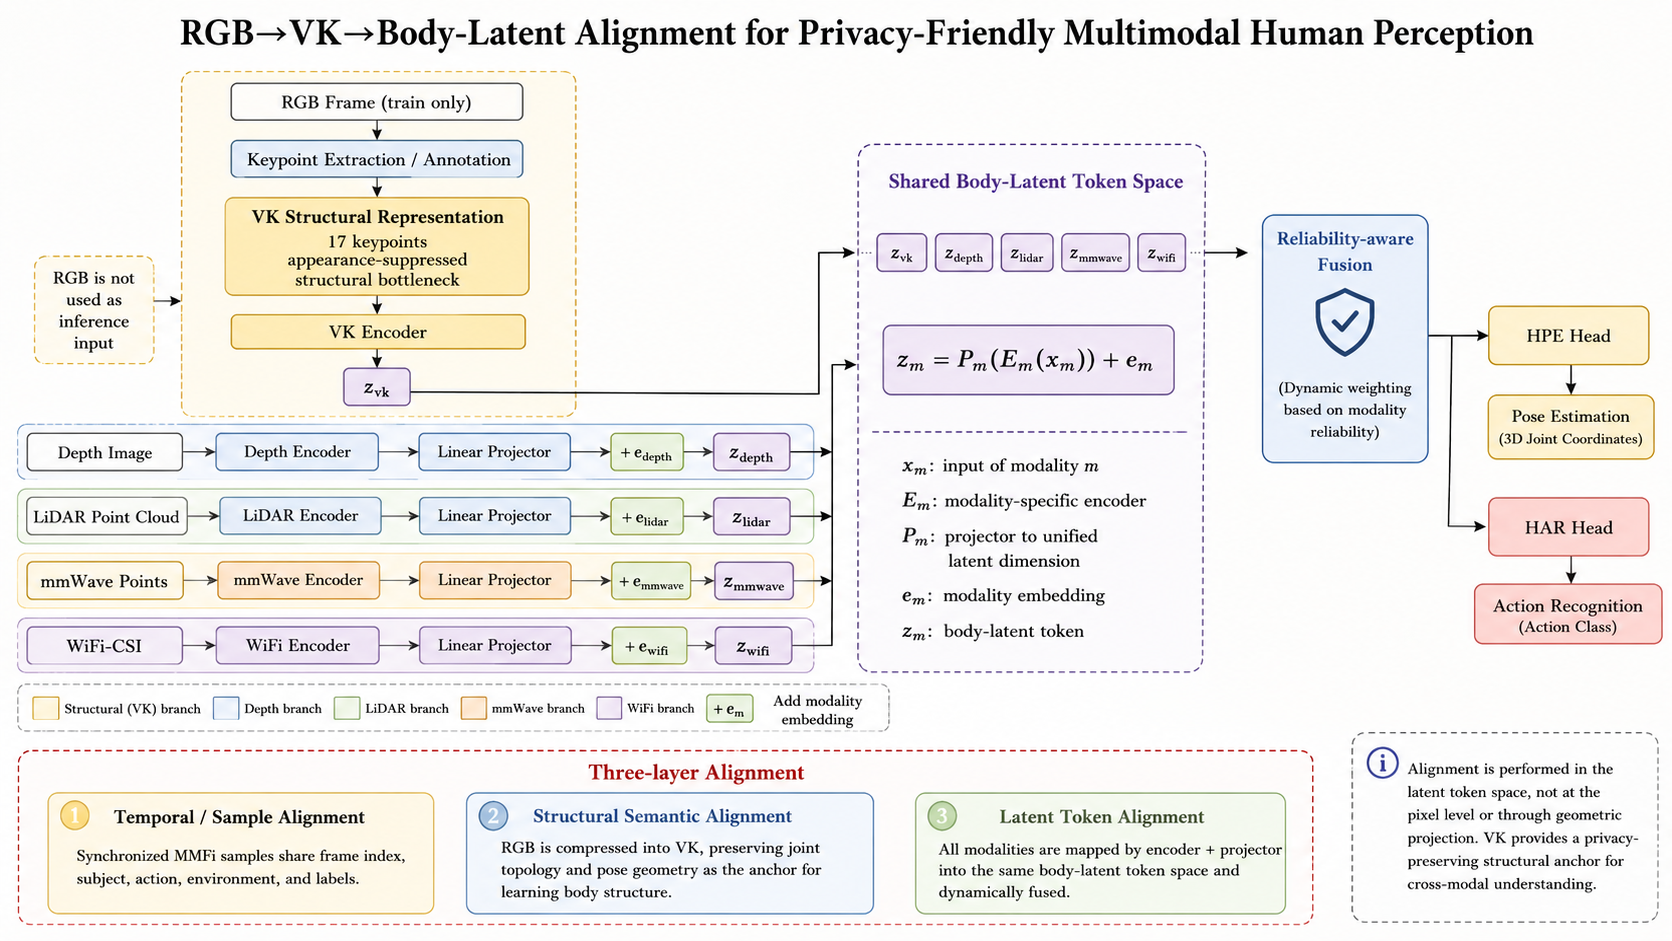
\includegraphics[width=0.98\linewidth]{../tables/1/fig1_rgb_vk_body_latent_alignment_current.png}
    \caption{Overall architecture of \method. RGB is used only during training to provide VK-based structural knowledge. The RGB frame is converted into VK keypoints, which serve as an appearance-suppressed body-structure bridge. VK and non-RGB sensor streams are processed by modality-specific encoders, represented in a shared body-latent space, fused by learned reliability-aware modality weights, and finally decoded by task-specific HPE and HAR heads.}
    \label{fig:framework}
\end{figure}

Fig.~\ref{fig:framework} summarizes the full processing chain. The left side describes training knowledge: raw RGB is not a deployed modality, but its structural information is compressed through VK. The middle part describes the variable-modality student: different samples can contain different available sensors, and each sensor is encoded into the same body-token dimension. The right side describes decision making: reliability-aware fusion produces a fused representation for either HPE or HAR. This organization reflects the paper's central claim that reduced visual exposure and missing-modality robustness are handled within one model pipeline.

\subsection{VK-anchored body-token encoding}

Each modality is encoded using a modality-specific extractor. VK is processed by a lightweight joint-aware encoder. The design avoids a large flattened mapping: each joint coordinate is lifted independently and then projected across joints to allow global interaction. Depth, LiDAR, mmWave, and WiFi-CSI features are encoded through corresponding modality backbones and projected into a shared body-token dimension.

Let $E_m(\cdot)$ denote the feature extractor for modality $m$ and $P_m(\cdot)$ denote the modality projector. The encoded modality token is
\begin{equation}
    \mathbf{z}_{m}=P_m(E_m(\mathbf{x}_{m}))+\mathbf{e}_{m},
\end{equation}
where $\mathbf{e}_{m}$ is a modality embedding. The embedding is necessary because the model receives variable modality subsets; it must know whether a token came from depth, LiDAR, mmWave, WiFi-CSI, or VK.

The modality-specific design also avoids forcing all sensor streams into the same raw preprocessing pipeline. Depth images, point clouds, radar points, WiFi-CSI sequences, and VK coordinates have different statistical properties. A shared encoder from raw inputs would either ignore these differences or require excessive preprocessing. Instead, \method{} uses specialized encoders and aligns features at the token level. This is the central mechanism that makes the framework more than a direct combination of dropout and attention: missing-modality learning occurs after heterogeneous inputs have been translated into a VK-anchored body-token space.

\subsection{Random missing-modality training}

Fig.~\ref{fig:missing_protocol} illustrates the training and evaluation protocol. At training time, modality subsets are randomly sampled. At evaluation time, all valid modality combinations are tested. This protocol turns missing-modality inference from a post-hoc stress test into a central training objective.

\begin{figure}[t]
    \centering
    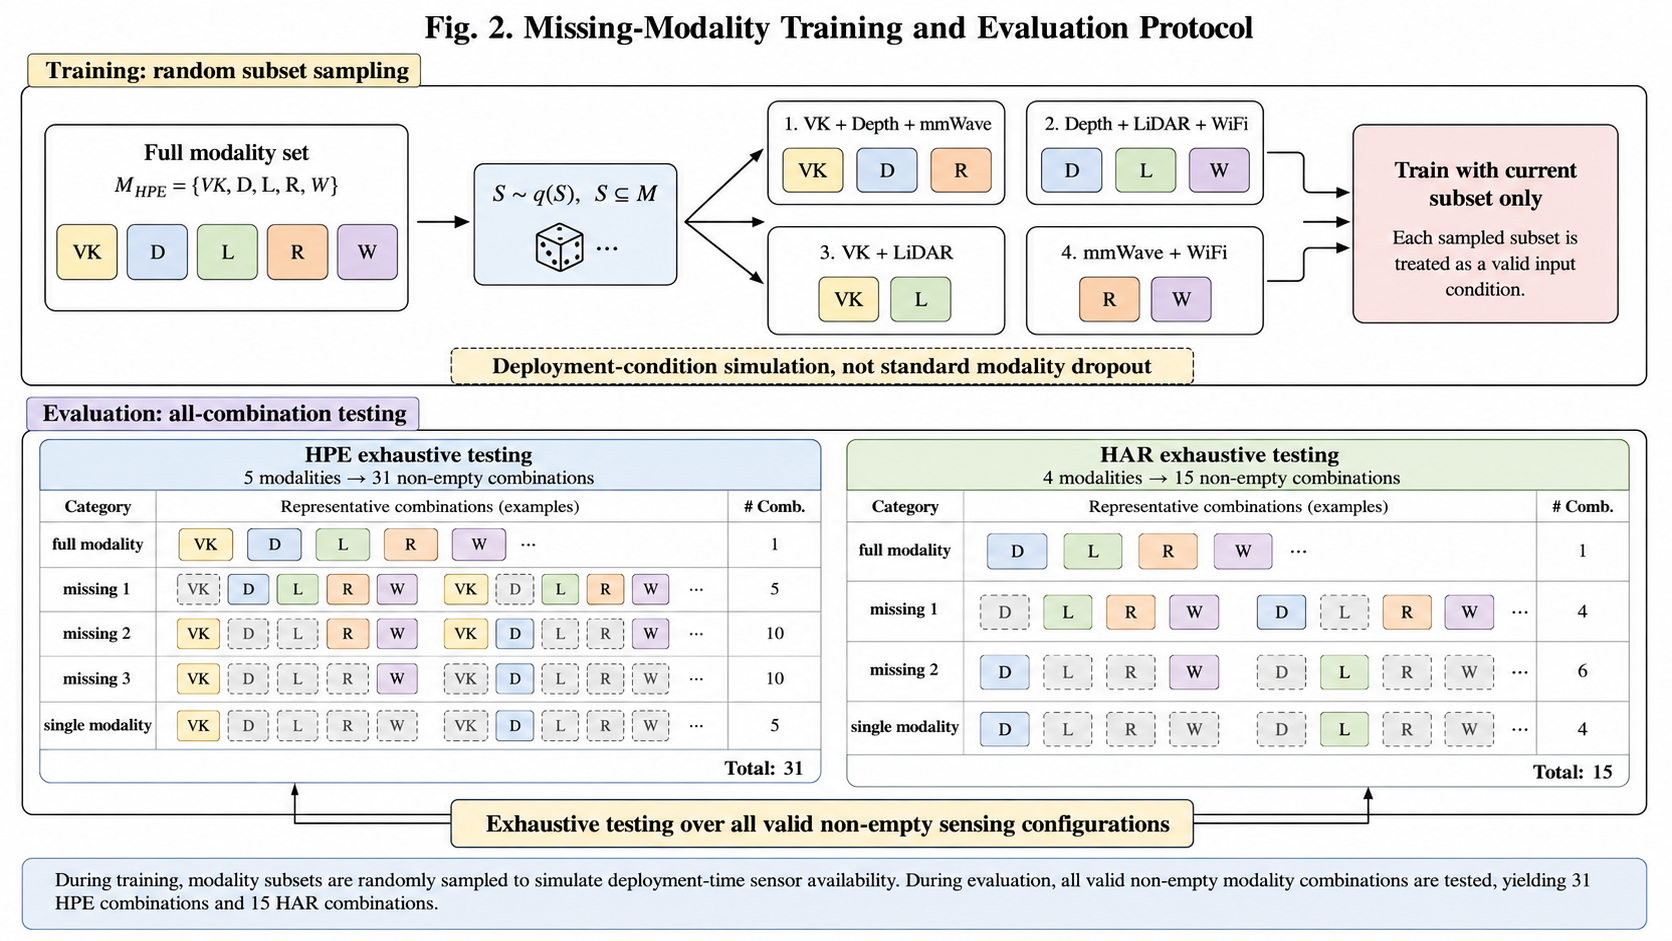
\includegraphics[width=0.98\linewidth]{../tables/1/fig2_missing_modality_protocol.png}
    \caption{Missing-modality training and evaluation protocol. During training, modality subsets are randomly sampled to simulate deployment-time sensor availability. During evaluation, all valid non-empty modality combinations are tested, yielding 31 HPE combinations and 15 HAR combinations.}
    \label{fig:missing_protocol}
\end{figure}

The expected training objective is
\begin{equation}
    \min_{\theta}\mathbb{E}_{(\mathbf{x},y)}
    \mathbb{E}_{\mathcal{S}\sim q(\mathcal{S})}
    \left[
    \mathcal{L}(f_{\theta}(\mathbf{x}_{\mathcal{S}},\mathcal{S}),y)
    \right],
\end{equation}
where $q(\mathcal{S})$ is the modality-subset sampling distribution.

The training distribution covers both mild and severe missing cases. If training samples only full-modality and one-missing-modality cases, the model may still fail when two or three modalities are unavailable. Conversely, if training overemphasizes single-modality cases, full-modality performance may suffer. The current implementation uses random missing counts such as one, two, and three missing modalities for student training. The evaluation is stricter than the sampling process because it reports every valid modality combination, including combinations that may be rare during training.

\subsection{Reliability-aware subset fusion}

For a given available subset $\mathcal{S}$, the model estimates a learned reliability proxy for each modality token. The normalized modality-contribution weight is
\begin{equation}
    \alpha_m =
    \frac{\exp(g(\mathbf{z}_{m}))}
    {\sum_{k\in\mathcal{S}}\exp(g(\mathbf{z}_{k}))},
    \quad m\in\mathcal{S}.
\end{equation}
The fused token is
\begin{equation}
    \mathbf{z}_{\mathrm{fuse}} =
    \sum_{m\in\mathcal{S}}\alpha_m\mathbf{z}_{m}.
\end{equation}
Uniform fusion is a special case with $\alpha_m=1/|\mathcal{S}|$. The ablation in Section~\ref{sec:ablation} directly tests whether learned reliability-aware weights are useful.

From an engineering perspective, reliability-aware fusion has two advantages. The first is performance: the model can downweight weak or missing-condition modalities. The second is diagnosability: exported alpha weights can reveal whether the model consistently depends on a modality or shifts its decision weight according to the input subset. The present manuscript includes ablation evidence, exported alpha-weight heatmaps, and subset-level reliability-performance correlation. These analyses support the use of the weights as task-level contribution proxies, but they are not interpreted as calibrated physical sensor reliability.

\subsection{Auxiliary teacher-student supervision}

The teacher uses full-modality information and privileged VK/RGB-derived supervision during training. The student is trained under missing subsets. Teacher-student supervision is auxiliary: it can stabilize subset learning, but the paper does not claim that it is the only or always-dominant source of improvement. For HPE, the student minimizes ground-truth pose regression and optional teacher pose matching:
\begin{equation}
    \mathcal{L}_{p}=
    \|\hat{\mathbf{Y}}^{p}_{s}-\mathbf{Y}^{p}\|_2^2
    +\lambda_{p}\|\hat{\mathbf{Y}}^{p}_{s}-\hat{\mathbf{Y}}^{p}_{t}\|_2^2
    +\lambda_{b}\mathcal{L}_{\mathrm{bone}}.
\end{equation}
For HAR, the student uses cross-entropy and logit distillation:
\begin{equation}
    \mathcal{L}_{a} =
    \mathrm{CE}(\hat{\mathbf{p}}_{s}^{a},y^{a})
    +\lambda_{a}\mathrm{KL}
    (\hat{\mathbf{p}}_{s}^{a}\|\hat{\mathbf{p}}_{t}^{a}).
\end{equation}

In the final system, the teacher is not the deployed model. The teacher is a training mechanism that provides stable supervision when the student is trained under incomplete inputs. This distinction is important because the teacher itself may not perform well when directly evaluated under missing combinations. The student is the model intended for missing-modality inference.

\subsection{Task-specific heads}

The HPE head regresses a $17\times3$ pose from the fused representation. The HAR head predicts a 27-class action distribution. The shared robustness mechanism is therefore task-agnostic, while the final output heads are task-specific.

\section{Experimental setup}

\subsection{Dataset and tasks}

Experiments are based on MMFi-style multimodal human perception data following the X-Fi/VK setting. HPE uses VK, depth, LiDAR, mmWave, and WiFi-CSI. HAR uses VK, depth, LiDAR, and mmWave in the current implementation. The dataset contains multiple environments, subjects, and actions, enabling random split, cross-scene, and cross-subject evaluation.

\subsection{Baselines and reproduced X-Fi/VK settings}

The reproduced X-Fi/VK outputs are treated as baselines. They are not counted as our method. This distinction is important for fair writing: the baseline provides a reference for prior VK-based multimodal perception, while \method{} adds VK-anchored body-token alignment, random missing-modality training, and reliability-aware fusion for robust deployment.

\subsection{Evaluation metrics}

HPE reports MSE, \mpjpe{}, and \pampjpe{}. The main tables emphasize \mpjpe{} because it is directly interpretable in millimeters. HAR reports accuracy and macro-F1 when available. For missing-modality robustness, we report average performance over all combinations and group performance by the number of missing modalities.

\subsection{Implementation details}

Training follows the project setting with 1000 training iterations per epoch where specified, while evaluation uses full validation sets unless explicitly stated. Checkpoints are selected by validation performance. The non-visual HPE student uses depth, LiDAR, mmWave, and WiFi-CSI; the non-visual HAR student uses depth, LiDAR, and mmWave. The same reliability-aware fusion principle is used across VK-enabled and non-visual variants.

The reported values are taken from local result files under the project directory. HPE main results are taken from \texttt{student\_vk\_random\_all\_combinations.csv}, \texttt{student\_nv\_random\_nonvisual\_combinations.csv}, and corresponding cross-scene/cross-subject files. The official HPE X-Fi/VK comparison is taken from the curated table file \texttt{legacy\_xfi/xfi\_hpe\_table1.csv}. HAR main results are taken from the analogous HAR result files, and the HAR reproduced baseline is taken from the \texttt{origin-XFI} outputs. Ablation results are taken from no-distillation and uniform-fusion result files. This traceability is important because the manuscript contains many experimental numbers; any number not traceable to a result file is marked as missing rather than invented.

\subsection{Figure organization}

The figure order follows the paper logic. Fig.~\ref{fig:framework} introduces the training-to-inference chain. Fig.~\ref{fig:missing_protocol} defines the missing-modality protocol. Fig.~\ref{fig:main_results} summarizes the main HPE/HAR performance. Fig.~\ref{fig:missing_robustness} shows robustness as missing severity increases. Fig.~\ref{fig:ablation} supports the module analysis. Fig.~\ref{fig:reliability_weights} visualizes exported reliability weights for representative missing-modality conditions. This ordering avoids the common problem of placing all figures at the end without narrative function.

\subsection{Result inclusion policy}

Because the project contains many result files, the manuscript follows a strict inclusion policy. Formal HPE and HAR student results are used as the main evidence. Reproduced X-Fi/VK results are used only as baselines. Ablation results are used only to support specific component claims. Super-Teacher results are used only as exploratory analysis. Extremely poor missing-combination results are not used to make the main method look worse or better; instead, they are summarized in limitation or appendix-level discussion when they reveal a meaningful failure mode.

This policy is necessary for two reasons. First, a paper with many experiments can become confusing if every output is presented with equal weight. The reader needs to know which results define the method, which results compare against prior work, and which results are exploratory. Second, EAAI reviewers are likely to judge whether the experimental evidence supports the stated engineering application. If Super-Teacher failure cases were placed in the main table, the main story would become ambiguous. If reproduced X-Fi/VK outputs were described as our own method, the contribution would be misleading. The result inclusion policy avoids both problems.

The formal main results are therefore: HPE Student-VK, HPE Student-NV, HAR Student-VK, and HAR Student-NV under random, cross-scene, and cross-subject protocols. The main ablations are: no-distillation and uniform fusion. Encoder ablations are acknowledged but not emphasized because some combinations collapse severely. Super-Teacher is discussed only as a training exploration.

\subsection{Protocol interpretation}

The random split evaluates whether the model can learn the overall mapping under the standard data partition. The cross-subject protocol evaluates whether the learned representation generalizes to unseen subjects. The cross-scene protocol evaluates whether it generalizes across environments. These protocols have different difficulty levels. The observed results show that cross-scene is the hardest for HPE and HAR averages, which is plausible because non-RGB signals can be strongly affected by room layout, sensor placement, and environmental reflection patterns. Cross-subject results are closer to random split, suggesting that the learned representation is less sensitive to subject identity than to environmental shift.

This interpretation turns raw numbers into engineering insight. The goal is not only to state that cross-scene performance is lower; the goal is to explain why this matters. A model intended for practical use cannot be evaluated only on random split. Scene shift exposes whether sensor fusion has learned general body cues or environment-specific correlations. The results suggest that \method{} improves robustness, but scene generalization remains a target for future work.

\section{Results and analysis}

\subsection{Main HPE results}

Table~\ref{tab:hpe_main} reports HPE results. The official X-Fi/VK table baseline obtains 103.70 mm average \mpjpe{} over 31 modality combinations. \method{} Student-VK obtains 75.18 mm, corresponding to a 27.51\% lower average error under the same all-combination summary. Student-NV obtains 84.68 mm over 15 non-visual combinations, demonstrating that the method remains effective when VK is removed at inference.

\begin{table*}[t]
\centering
\caption{Main HPE results. Lower \mpjpe{} is better. ``Official X-Fi/VK table'' is a baseline, not our contribution.}
\label{tab:hpe_main}
\begin{adjustbox}{width=\textwidth}
\begin{tabular}{llcccccc}
\toprule
Method & Role & Inference modalities & RGB inference & Protocol & Combinations & Avg. \mpjpe{} (mm) & Full \mpjpe{} (mm) \\
\midrule
Official X-Fi/VK table & Baseline & VK+D+L+R+W & No & Random & 31 & 103.70 & 83.70 \\
\method{} Student-VK & Ours & VK+D+L+R+W & No & Random & 31 & \textbf{75.18} & 50.17 \\
\method{} Student-NV & Ours & D+L+R+W & No & Random & 15 & 84.68 & 51.03 \\
\method{} Student-VK & Ours & VK+D+L+R+W & No & Cross-scene & 31 & 142.02 & 71.71 \\
\method{} Student-NV & Ours & D+L+R+W & No & Cross-scene & 15 & 153.89 & 78.96 \\
\method{} Student-VK & Ours & VK+D+L+R+W & No & Cross-subject & 31 & 78.57 & 49.88 \\
\method{} Student-NV & Ours & D+L+R+W & No & Cross-subject & 15 & 90.74 & 52.45 \\
\bottomrule
\end{tabular}
\end{adjustbox}
\end{table*}

The random-split Student-VK result shows the benefit of VK as a structural bridge. The Student-NV result is particularly important for reduced-exposure inference because it removes VK as well as raw RGB. Cross-scene results are weaker than random and cross-subject results, indicating that scene shift remains a major challenge.

Several observations follow from Table~\ref{tab:hpe_main}. First, Student-VK improves the average all-combination \mpjpe{} over the official X-Fi/VK table baseline, and the margin is interpreted as an engineering robustness improvement rather than an order-of-magnitude breakthrough. The reduction from 103.70 mm to 75.18 mm is substantial and credible; a much larger comparison against a weak local reproduction is not used as the main claim. Second, Student-NV is only moderately worse than Student-VK in random split full-modality inference (51.03 mm versus 50.17 mm). This suggests that non-visual modalities contain enough complementary information when all are available. Third, cross-scene evaluation is much harder than cross-subject evaluation. Student-VK increases from 75.18 mm average \mpjpe{} in random split to 142.02 mm in cross-scene evaluation, while cross-subject performance remains 78.57 mm. This pattern implies that environmental shift affects sensor distributions more strongly than subject identity shift in the current setting.

The HPE results also clarify the role of VK. VK helps average robustness, but the non-visual variant remains competitive enough to support a stricter reduced-exposure interpretation. Therefore, VK is framed as a structural bridge and optional inference modality, while non-visual inference is a separate supported setting.

\paragraph{Comparison with reproduced baseline.}
The reproduced baseline is useful because it answers a practical question: what happens if a VK/X-Fi style model is evaluated under all missing combinations without the proposed missing-modality adaptation? The high average \mpjpe{} indicates that full-modality success does not automatically transfer to missing-modality success. This is one of the paper's central engineering messages. It also explains why the main comparison uses all-combination averages rather than only the full-modality row.

\paragraph{Non-visual setting.}
The Student-NV setting is stricter than Student-VK because it removes VK at inference. In HPE, Student-NV obtains 84.68 mm average \mpjpe{} and 51.03 mm full non-visual \mpjpe{}. The full non-visual result is close to Student-VK full-modality performance, but the average is worse because severe missing cases are harder without VK. This distinction is central to the interpretation: non-visual inference is feasible, while VK still provides useful structural information when allowed.

\subsection{Main HAR results}

Table~\ref{tab:har_main} reports HAR results. The official/reproduced X-Fi/VK baseline obtains 62.46\% average accuracy over 15 combinations. \method{} Student-VK obtains 85.15\% average accuracy and 96.56\% full-modality accuracy. Student-NV obtains 80.62\% average accuracy across non-visual combinations and 96.12\% full non-visual accuracy.

\begin{table*}[t]
\centering
\caption{Main HAR results. Higher accuracy is better.}
\label{tab:har_main}
\begin{adjustbox}{width=\textwidth}
\begin{tabular}{llcccccc}
\toprule
Method & Role & Inference modalities & RGB inference & Protocol & Combinations & Avg. accuracy (\%) & Full accuracy (\%) \\
\midrule
Official/reproduced X-Fi/VK & Baseline & VK+D+L+R & No & Random & 15 & 62.46 & 72.20 \\
\method{} Student-VK & Ours & VK+D+L+R & No & Random & 15 & \textbf{85.15} & \textbf{96.56} \\
\method{} Student-NV & Ours & D+L+R & No & Random & 7 & 80.62 & 96.12 \\
\method{} Student-VK & Ours & VK+D+L+R & No & Cross-scene & 15 & 80.61 & 95.25 \\
\method{} Student-NV & Ours & D+L+R & No & Cross-scene & 7 & 76.70 & 95.41 \\
\method{} Student-VK & Ours & VK+D+L+R & No & Cross-subject & 15 & 85.30 & 96.12 \\
\method{} Student-NV & Ours & D+L+R & No & Cross-subject & 7 & 81.26 & 95.70 \\
\bottomrule
\end{tabular}
\end{adjustbox}
\end{table*}

HAR results support the application value of the framework beyond pose regression. They show that the same missing-modality robustness strategy also improves action recognition.

HAR results also reveal a different robustness profile from HPE. Full-modality accuracy is high for both Student-VK and Student-NV, indicating that action classes can be recognized well when sufficient non-visual evidence is available. The average over all combinations is lower because single-modality and severe-missing cases are difficult. The official/reproduced baseline average of 62.46\% shows that fixed or insufficiently adapted fusion is not enough for all-combination HAR. Student-VK improves the average to 85.15\%, and Student-NV still reaches 80.62\%, which is important for inference settings without VK.

Cross-scene HAR remains strong in full modality: Student-VK obtains 95.25\% full accuracy and Student-NV obtains 95.41\%. However, the average across combinations drops to 80.61\% and 76.70\%, respectively. This suggests that full sensor availability can compensate for scene shift, but missing sensors make generalization harder. This is a useful engineering finding: robust deployment cannot rely on a single sensor in unseen scenes.

\paragraph{Action recognition under non-visual sensing.}
HAR Student-NV is important because action recognition can often be performed from motion and geometry cues rather than visual appearance. The 96.12\% full non-visual accuracy indicates that depth, LiDAR, and mmWave together provide strong semantic information. The lower 80.62\% average across non-visual combinations shows that the challenge is not full non-visual recognition but robust recognition when only a subset remains. This again supports the missing-modality focus of the paper.

\paragraph{Why HAR strengthens the paper.}
If the paper reported only HPE, reviewers could interpret \method{} as a pose-specific engineering solution. HAR shows that the same robust fusion design also supports action semantics. Conversely, if the paper reported only HAR, the method would lack fine-grained body-structure validation. Reporting both tasks makes the work more convincing as a multimodal human perception framework.

\subsection{Fair missing-modality baseline comparison}
\label{sec:fair_baseline}

Table~\ref{tab:fair_baseline} addresses a key fairness concern: the proposed model is not judged only against a prior model that was not adapted to missing modalities. We therefore report official/reproduced X-Fi/VK baselines together with stronger internal baselines, including a full-modality model evaluated under missing combinations, uniform fusion, and no-distillation variants. This table changes the interpretation of the results. The method is not presented as simply defeating a weak reproduction; instead, it is evaluated against missing-trained and fusion-controlled variants.

\begin{table*}[t]
\centering
\caption{Fair missing-modality baseline comparison. HPE uses average \mpjpe{} in mm over combinations, where lower is better. HAR uses average accuracy in \%, where higher is better.}
\label{tab:fair_baseline}
\scriptsize
\begin{adjustbox}{width=\textwidth}
\begin{tabular}{llcccl}
\toprule
Task & Method & Missing-modality training & Adaptive fusion & KD & Avg. / full metric and interpretation \\
\midrule
HPE & Official X-Fi/VK table & No & X-fusion / reported & No & 103.70 / 83.70 mm; external reference baseline \\
HPE & Full-modality baseline under missing test & No & Standard fusion & No & 617.17 / 49.14 mm; full-input training is brittle under missing inputs \\
HPE & Uniform-fusion ablation & Yes & Uniform weights & Yes & 82.77 / 52.28 mm; tests learned fusion beyond missing training \\
HPE & w/o KD ablation & Yes & Yes & No & 72.68 / 48.83 mm; HPE distillation is task-dependent \\
HPE & \method{} Student-VK & Yes & Yes & Auxiliary & 75.18 / 50.17 mm; main VK-enabled student \\
HPE & \method{} Student-NV & Yes & Yes & Auxiliary & 84.68 / 51.03 mm; stricter non-visual student \\
\midrule
HAR & Official/reproduced X-Fi/VK & No & X-fusion / reported & No & 62.46 / 72.20\%; external reference baseline \\
HAR & Full-modality teacher under missing test & No & Standard full-modality teacher & No & 66.25 / 95.57\%; full teacher is not missing-robust \\
HAR & Uniform-fusion ablation & Yes & Uniform weights & Yes & 67.46 / 95.39\%; equal weighting is weak under missing inputs \\
HAR & w/o KD ablation & Yes & Yes & No & 82.86 / 95.99\%; KD provides auxiliary benefit \\
HAR & \method{} Student-VK & Yes & Yes & Auxiliary & 85.15 / 96.56\%; main VK-enabled student \\
HAR & \method{} Student-NV & Yes & Yes & Auxiliary & 80.62 / 96.12\%; stricter non-visual student \\
\bottomrule
\end{tabular}
\end{adjustbox}
\end{table*}

The fair comparison leads to three conclusions. First, full-modality models can have strong full-input endpoints but fail badly when evaluated under missing combinations, especially in HPE. Second, reliability-aware fusion is more important than distillation in the current evidence: uniform fusion is consistently weaker, whereas the HPE no-KD variant remains competitive. Third, Student-NV is not designed to outperform Student-VK in every setting; it provides a stricter inference mode when VK is unavailable or disallowed.

\begin{figure}[t]
    \centering
    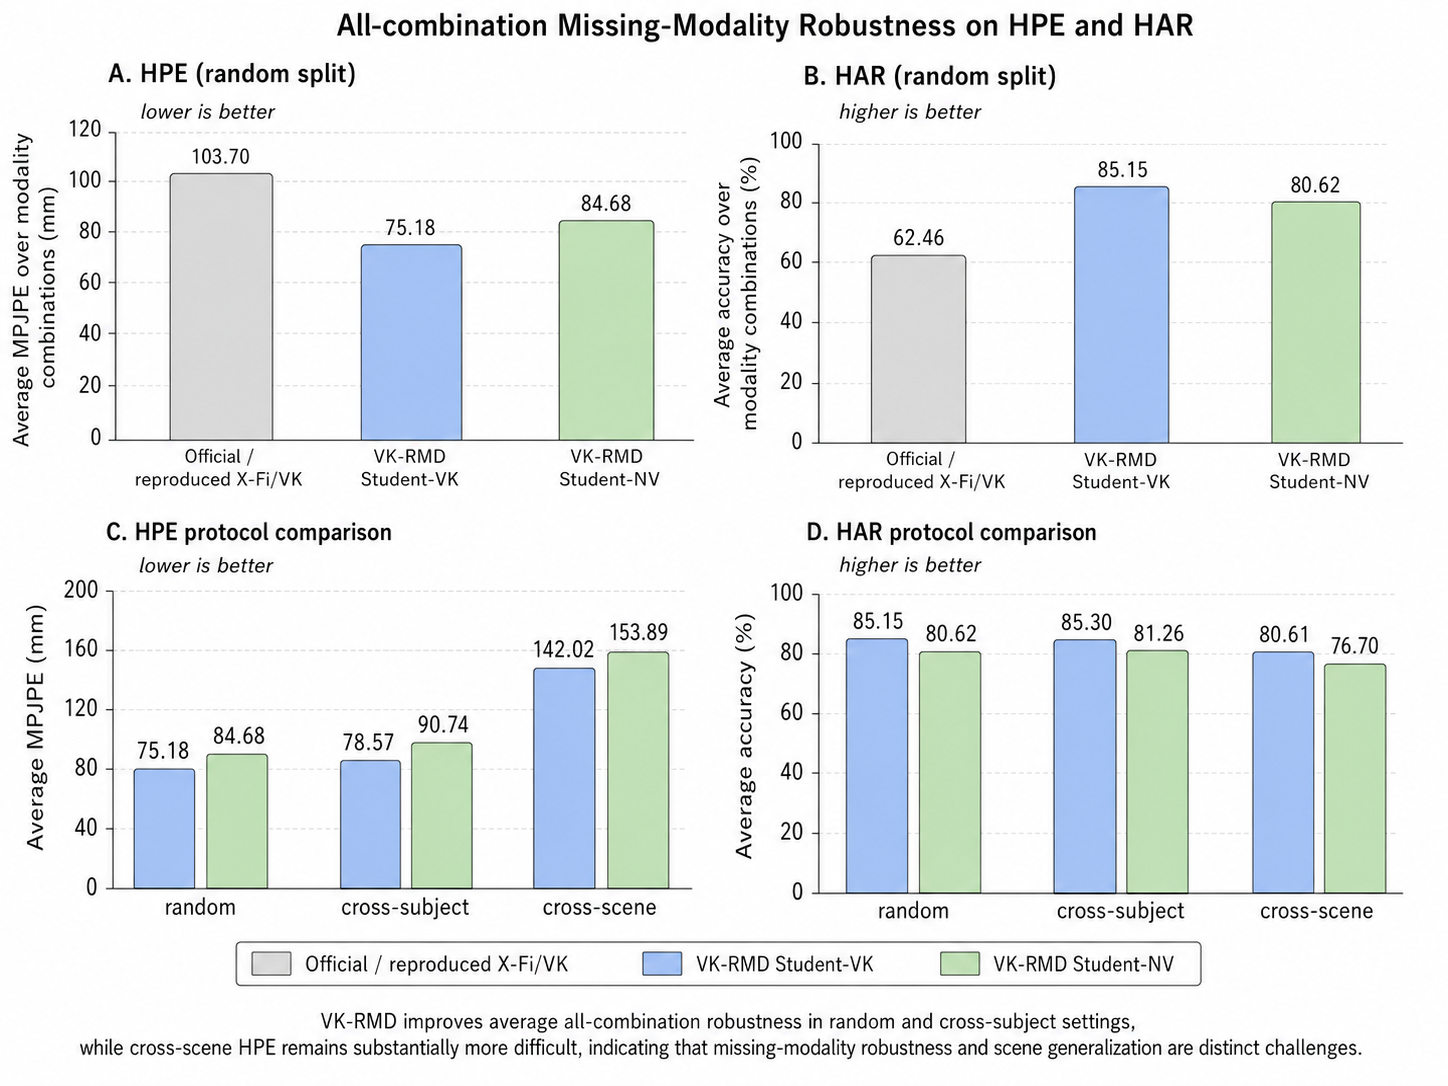
\includegraphics[width=0.98\linewidth]{../tables/1/fig3_main_hpe_har_results.png}
    \caption{Main HPE and HAR results under arbitrary modality combinations. Panels A and B compare VK-RMD with official/reproduced X-Fi/VK baselines under the random split. Panels C and D report random, cross-subject, and cross-scene protocols for Student-VK and Student-NV, showing that cross-scene HPE remains the most difficult setting.}
    \label{fig:main_results}
\end{figure}

\subsection{Robustness under missing modalities}
\label{sec:missing}

Table~\ref{tab:missing_group} groups results by the number of missing modalities. HPE Student-VK degrades from 50.17 mm with all modalities to 78.10 mm when three modalities are missing, and to 124.76 mm in single-modality inference. Student-NV follows a similar pattern. HAR Student-VK remains above 87\% accuracy with two missing modalities, but drops to 70.00\% in single-modality inference. HAR Student-NV drops more sharply when only one non-visual modality remains.

\begin{table*}[t]
\centering
\caption{Grouped missing-modality robustness. HPE reports \mpjpe{} in mm; HAR reports accuracy in \%.}
\label{tab:missing_group}
\begin{adjustbox}{width=\textwidth}
\begin{tabular}{lcccccc}
\toprule
Task/model & Metric & Missing 0 & Missing 1 & Missing 2 & Missing 3 & Missing 4 \\
\midrule
HPE Student-VK & \mpjpe{} $\downarrow$ & 50.17 & 53.55 & 60.78 & 78.10 & 124.76 \\
HPE Student-NV & \mpjpe{} $\downarrow$ & 51.03 & 61.32 & 79.43 & 124.32 & -- \\
HAR Student-VK & Accuracy $\uparrow$ & 96.56 & 93.83 & 87.55 & 70.00 & -- \\
HAR Student-NV & Accuracy $\uparrow$ & 96.12 & 90.05 & 66.02 & -- & -- \\
\bottomrule
\end{tabular}
\end{adjustbox}
\end{table*}

\begin{figure}[t]
    \centering
    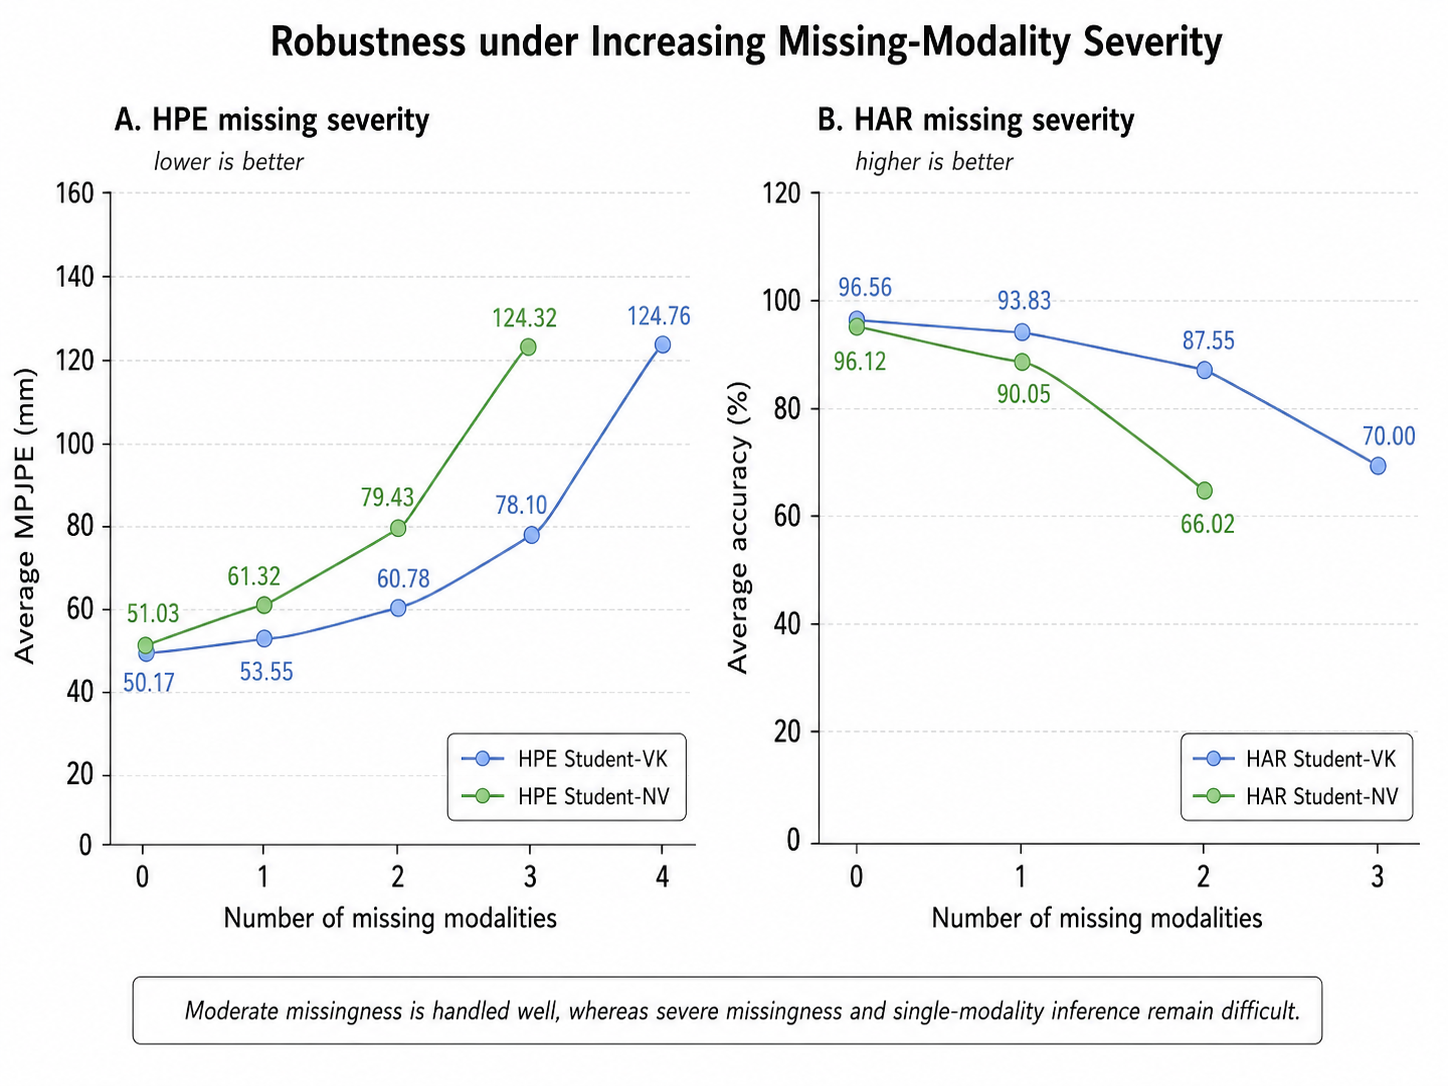
\includegraphics[width=0.98\linewidth]{../tables/1/fig4_missing_modality_severity.png}
    \caption{Robustness under increasing missing-modality severity. The curves summarize grouped missing-modality results from Table~\ref{tab:missing_group}. Moderate missingness is handled well, whereas severe missingness and single-modality inference remain difficult.}
    \label{fig:missing_robustness}
\end{figure}

The degradation trend is expected: fewer modalities provide less complementary evidence. The key observation is not that single-modality inference is always strong, but that the trained student degrades gradually and remains substantially more robust than fixed full-modality baselines in all-combination evaluation.

The grouped analysis is more informative than reporting only the overall average. For HPE Student-VK, missing one modality increases \mpjpe{} only from 50.17 mm to 53.55 mm. Missing two modalities increases it to 60.78 mm. This indicates that moderate missingness is well handled. The larger jump appears when only one or two modalities remain. For HAR Student-VK, missing one modality still gives 93.83\% accuracy, and missing two modalities gives 87.55\%. Again, severe missingness is the main remaining difficulty.

For Student-NV, the trend is similar but generally weaker in severe cases. This is expected because non-visual settings remove VK, one of the most structurally direct representations. The key value of Student-NV is therefore not that it always matches Student-VK, but that it provides a stricter non-visual inference option with strong full non-visual performance and reasonable all-combination averages.

\paragraph{Moderate missingness versus severe missingness.}
The results suggest two regimes. In the moderate regime, one or two modalities are missing. Here, the model typically remains strong because complementary sensors are still available. In the severe regime, only one or two modalities remain. Performance decreases more sharply because each modality alone captures only part of the human state. This distinction is important for application planning. The proposed method can provide strong robustness for common missing cases, while severe single-modality scenarios may require additional modality-specific enhancement or confidence-based rejection.

\paragraph{Failure modes.}
The most difficult combinations are those relying on weak single modalities. WiFi-CSI and LiDAR alone can be challenging for precise HPE. LiDAR-only HAR is also weak in several protocols. These failures are not hidden in the project results, but they are not placed in the main abstract-level claims because they represent expected edge cases. The appendix reports full combination tables to make these failure modes traceable.

Table~\ref{tab:leave_one} further reports leave-one-modality-out degradation from the full Student-VK setting. The result is useful because it separates two concepts that are often conflated: a modality can be available, but its removal may or may not strongly affect the final task. For HPE, removing depth causes the largest degradation among one-missing cases, increasing \mpjpe{} by 14.07 mm. Removing WiFi-CSI causes almost no degradation in the full five-modality setting, which is consistent with the weaker WiFi-only pose results. For HAR, removing mmWave causes the largest accuracy drop, followed by depth. This task-dependent pattern supports the need for adaptive fusion rather than a fixed modality preference.

\begin{table*}[t]
\centering
\caption{Leave-one-modality-out degradation from the full Student-VK setting. HPE degradation is an increase in \mpjpe{}; HAR degradation is a decrease in accuracy.}
\label{tab:leave_one}
\begin{adjustbox}{width=\textwidth}
\begin{tabular}{llcccc}
\toprule
Task & Missing modality & Full metric & Leave-one-out metric & Degradation & Interpretation \\
\midrule
HPE & VK & 50.17 mm & 51.78 mm & 1.61 mm & VK helps, but non-RGB sensors compensate in full setting \\
HPE & Depth & 50.17 mm & 64.25 mm & 14.07 mm & Depth is the most influential HPE modality here \\
HPE & LiDAR & 50.17 mm & 50.41 mm & 0.24 mm & Limited marginal loss when other modalities remain \\
HPE & mmWave & 50.17 mm & 51.05 mm & 0.88 mm & Mild marginal loss under full setting \\
HPE & WiFi-CSI & 50.17 mm & 50.25 mm & 0.08 mm & Weak marginal effect for HPE full setting \\
\midrule
HAR & VK & 96.56\% & 96.44\% & 0.12 pp & Minor effect when depth/LiDAR/mmWave remain \\
HAR & Depth & 96.56\% & 92.73\% & 3.83 pp & Depth contributes to HAR robustness \\
HAR & LiDAR & 96.56\% & 96.56\% & 0.00 pp & Low marginal loss under full setting \\
HAR & mmWave & 96.56\% & 89.62\% & 6.94 pp & mmWave is most influential for HAR here \\
\bottomrule
\end{tabular}
\end{adjustbox}
\end{table*}

\subsection{Ablation study}
\label{sec:ablation}

Table~\ref{tab:ablation} summarizes ablation results. For HPE, uniform fusion increases average \mpjpe{} from 75.18 mm to 82.77 mm. For HAR, uniform fusion reduces average accuracy from 85.15\% to 67.46\%. This strong HAR gap shows that reliability-aware fusion is not merely a cosmetic module; it is essential when modalities have different quality and availability.

\begin{table*}[t]
\centering
\caption{Ablation results. HPE reports average \mpjpe{} over 31 combinations; HAR reports average accuracy over 15 combinations.}
\label{tab:ablation}
\begin{adjustbox}{width=\textwidth}
\begin{tabular}{llccc}
\toprule
Task & Setting & Avg. metric & Full metric & Interpretation \\
\midrule
HPE & \method{} Student-VK & 75.18 mm & 50.17 mm & Main model \\
HPE & w/o distillation & 72.68 mm & 48.83 mm & HPE KD gain is not consistent across all metrics; claim cautiously \\
HPE & Uniform fusion & 82.77 mm & 52.28 mm & Reliability fusion improves robustness \\
HPE & Simple MLP VK encoder & 503.74 mm & 77.69 mm & Severe missing-combination degradation; appendix-level detail \\
HPE & Skeleton prompt encoder & 1000.80 mm & 55.07 mm & Severe missing-combination degradation; appendix-level detail \\
HAR & \method{} Student-VK & 85.15\% & 96.56\% & Main model \\
HAR & w/o distillation & 82.86\% & 95.99\% & Distillation modestly improves average robustness \\
HAR & Uniform fusion & 67.46\% & 95.39\% & Reliability fusion is critical under missing modalities \\
\bottomrule
\end{tabular}
\end{adjustbox}
\end{table*}

\begin{figure}[t]
    \centering
    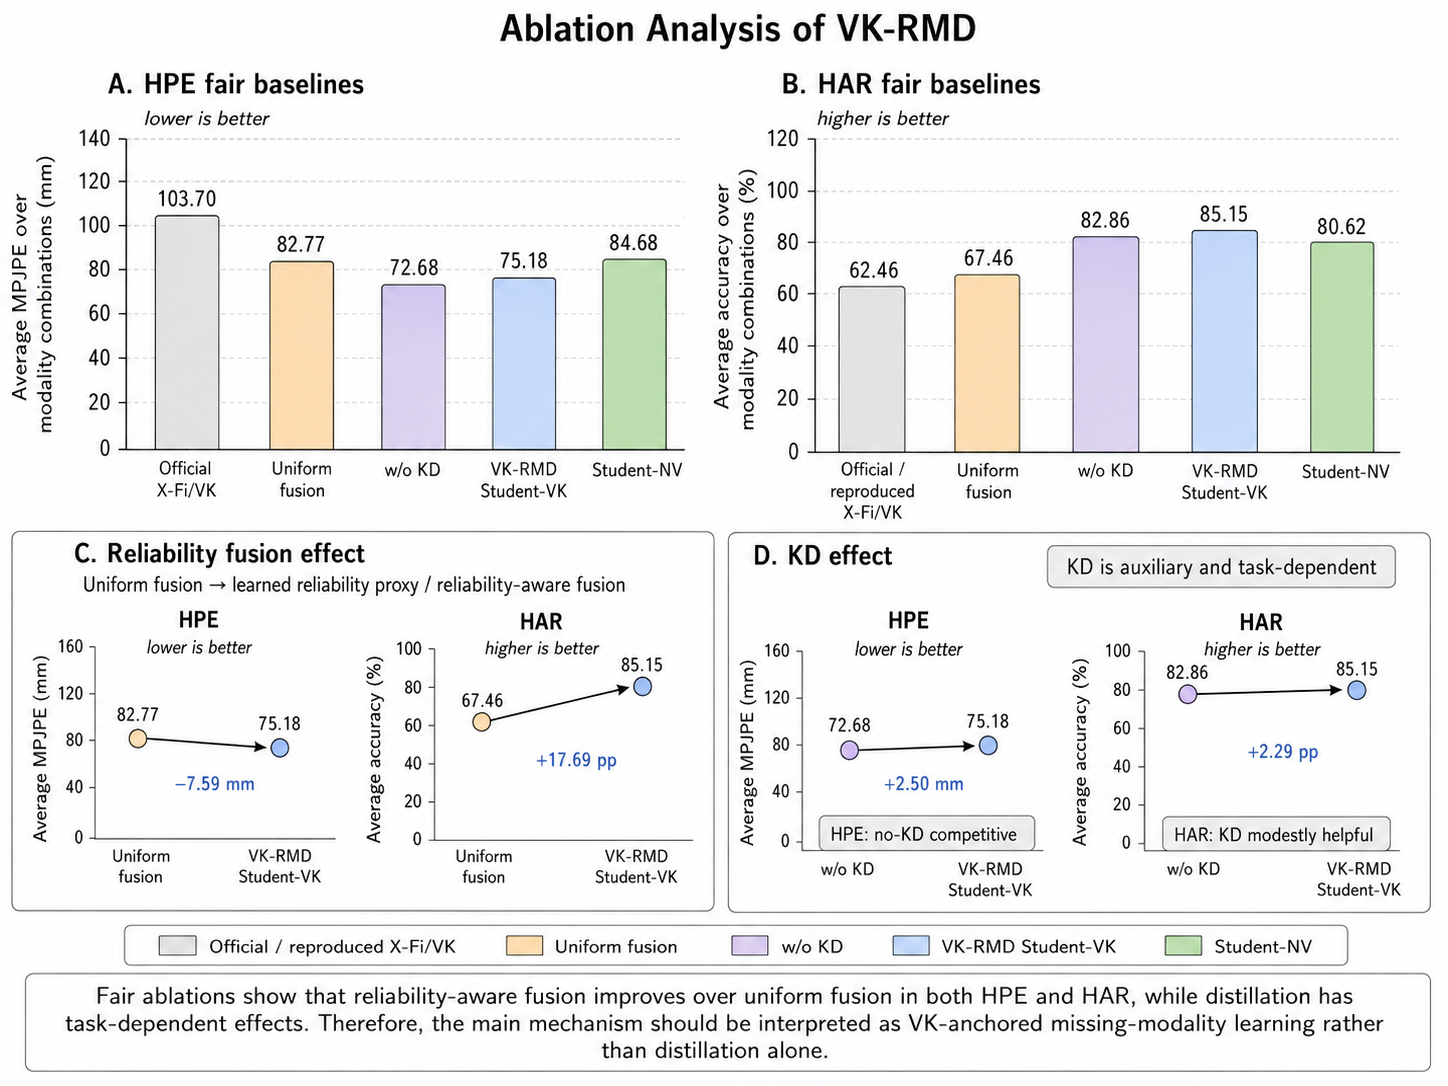
\includegraphics[width=0.98\linewidth]{../tables/1/fig5_ablation_fair_baseline.png}
    \caption{Ablation and fair-baseline analysis of \method. Reliability-aware fusion improves over uniform fusion in both HPE and HAR, while distillation has task-dependent effects. HPE no-distillation remains competitive, so the main mechanism is interpreted as VK-anchored missing-modality learning rather than distillation alone.}
    \label{fig:ablation}
\end{figure}

The ablation results lead to two important observations. First, reliability-aware fusion is a central and empirically supported component. The performance drop under uniform fusion is clear, especially in HAR. Second, distillation is part of the training framework rather than the only explanation for performance. The HPE no-distillation result is slightly better than the full model in the current all-combination average, which prevents a broad claim that distillation always improves HPE. This does not invalidate the framework; it defines distillation as an auxiliary and task-dependent component.

For an engineering application paper, this kind of nuanced ablation is useful. Every module does not need to improve every metric monotonically; the analysis identifies which design choices are essential, which are task-dependent, and which require further study. In our case, reliability fusion is essential, missing-modality training is central, and distillation is useful but interpreted task-dependently.

Table~\ref{tab:hpe_kd_variants} further breaks down the HPE distillation variants using full-modality endpoint evaluation. Output-level KD gives the lowest full-modality \mpjpe{} among these variants (47.62 mm), while token and bone variants do not monotonically improve the full-modality endpoint. This result is reported to make the distillation claim precise: KD is part of the training design and can improve specific settings, but the strongest and most consistent robustness evidence comes from missing-modality training and reliability-aware fusion.

\begin{table}[t]
\centering
\caption{HPE distillation-variant endpoint results under full-modality evaluation. Lower is better.}
\label{tab:hpe_kd_variants}
\begin{tabular}{lccc}
\toprule
Variant & \mpjpe{} (mm) & \pampjpe{} (mm) & MSE \\
\midrule
No KD & 48.83 & 32.51 & 0.001396 \\
Output KD & 47.62 & 32.15 & 0.001365 \\
Output+token KD & 48.76 & 33.24 & 0.001408 \\
Output+bone KD & 49.34 & 33.38 & 0.001417 \\
Full structural KD & 49.20 & 34.63 & 0.001422 \\
\bottomrule
\end{tabular}
\end{table}

Table~\ref{tab:endpoint_sanity} summarizes additional full-modality endpoint results from the final checkpoints. These values are not a replacement for all-combination robustness metrics, but they help verify that the trained models did not trade away normal full-input performance. For HPE, Student-VK and Student-NV remain close to the full-modality teacher in the random split. For HAR, Student-VK and Student-NV slightly exceed the full-modality teacher in random-split endpoint accuracy, while cross-scene and cross-subject endpoint results remain above 95\% for the student variants.

\begin{table*}[t]
\centering
\caption{Full-modality endpoint sanity checks from final checkpoints. HPE uses \mpjpe{}; HAR uses accuracy. These endpoint values complement, but do not replace, all-combination evaluation.}
\label{tab:endpoint_sanity}
\scriptsize
\begin{adjustbox}{width=\textwidth}
\begin{tabular}{llccc|llccc}
\toprule
Task & Model/protocol & Main metric & Secondary & Loss/MSE & Task & Model/protocol & Main metric & Secondary & Loss/MSE \\
\midrule
HPE & Teacher, random & 48.45 mm & 33.06 mm & 0.001392 & HAR & Teacher, random & 95.57\% & 95.56\% F1 & 0.2033 \\
HPE & Baseline full, random & 49.14 mm & 33.48 mm & 0.001415 & HAR & Student-VK, random & 96.54\% & 96.53\% F1 & 0.1627 \\
HPE & Student-VK, random & 50.17 mm & 33.48 mm & 0.001459 & HAR & Student-NV, random & 96.12\% & 96.13\% F1 & 0.1939 \\
HPE & Student-NV, random & 51.03 mm & 35.69 mm & 0.001493 & HAR & w/o distillation & 95.97\% & 95.95\% F1 & 0.2089 \\
HPE & Teacher, cross-scene & 76.06 mm & 37.89 mm & 0.002501 & HAR & Uniform fusion & 95.40\% & 95.40\% F1 & 0.1873 \\
HPE & Student-VK, cross-scene & 71.70 mm & 47.74 mm & 0.002393 & HAR & Student-VK, cross-scene & 96.12\% & 96.10\% F1 & 0.3624 \\
HPE & Student-VK, cross-subject & 49.88 mm & 32.35 mm & 0.001230 & HAR & Student-NV, cross-scene & 95.41\% & 95.40\% F1 & 0.3327 \\
HPE & Student-NV, cross-subject & 52.46 mm & 34.13 mm & 0.001367 & HAR & Student-NV, cross-subject & 95.66\% & 95.64\% F1 & 0.3926 \\
\bottomrule
\end{tabular}
\end{adjustbox}
\end{table*}

\subsection{Reliability-aware fusion analysis}

Reliability-aware fusion is supported by the uniform-fusion ablation, the exported reliability weights, and subset-level correlation analysis. Fig.~\ref{fig:reliability_weights} visualizes the average normalized weights assigned to each available modality for HPE Student-VK and HAR Student-VK. The heatmap is not interpreted as a complete explanation of the neural model or as calibrated physical sensor reliability. It verifies that the fusion module does not collapse into fixed uniform averaging.

\begin{figure}[t]
    \centering
    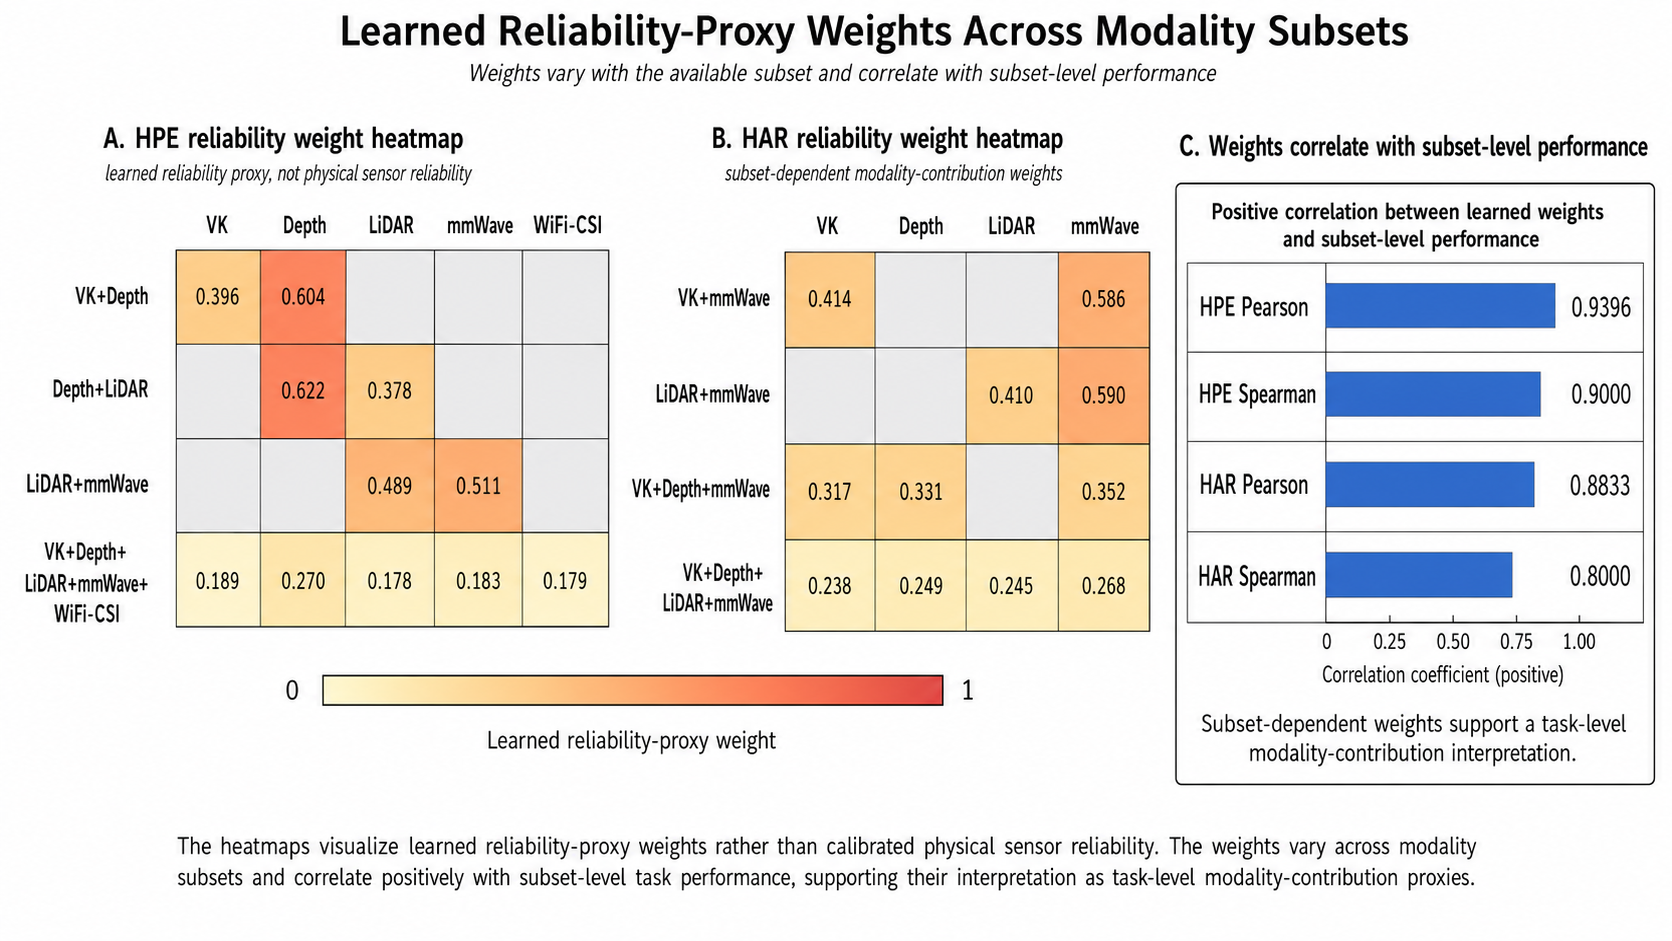
\includegraphics[width=0.98\linewidth]{../tables/1/fig6_reliability_proxy_weights.png}
    \caption{Learned reliability-proxy weights across modality subsets. The heatmaps visualize subset-dependent modality-contribution weights for HPE and HAR, and the correlation panel reports positive associations between learned weights and subset-level task performance. The weights are interpreted as task-level contribution proxies rather than calibrated physical sensor reliability.}
    \label{fig:reliability_weights}
\end{figure}

Table~\ref{tab:reliability_examples} reports representative averages from the same CSV files. For HPE, the model assigns more weight to depth than VK in the VK+Depth pair (0.604 versus 0.396), and also favors depth in Depth+LiDAR (0.622 versus 0.378). In the full five-modality HPE setting, weights are more distributed, with depth remaining the largest contributor (0.270). For HAR, mmWave receives larger weights than VK or LiDAR in combinations containing mmWave, such as VK+mmWave (0.586) and LiDAR+mmWave (0.590). These patterns are consistent with the performance tables, where depth and mmWave often provide strong complementary evidence. The analysis supports the engineering claim that reliability-aware fusion adapts to the available sensor subset.

\begin{table*}[t]
\centering
\caption{Representative exported reliability weights for Student-VK. Values are averaged over validation samples. Missing entries indicate unavailable modalities.}
\label{tab:reliability_examples}
\scriptsize
\begin{adjustbox}{width=\textwidth}
\begin{tabular}{llccccc}
\toprule
Task & Modality set & VK & Depth & LiDAR & mmWave & WiFi-CSI \\
\midrule
HPE & VK+Depth & 0.396 & 0.604 & -- & -- & -- \\
HPE & Depth+LiDAR & -- & 0.622 & 0.378 & -- & -- \\
HPE & LiDAR+mmWave & -- & -- & 0.489 & 0.511 & -- \\
HPE & VK+Depth+LiDAR & 0.288 & 0.436 & 0.276 & -- & -- \\
HPE & VK+Depth+LiDAR+mmWave+WiFi-CSI & 0.189 & 0.270 & 0.178 & 0.183 & 0.179 \\
\midrule
HAR & VK+mmWave & 0.414 & -- & -- & 0.586 & -- \\
HAR & LiDAR+mmWave & -- & -- & 0.410 & 0.590 & -- \\
HAR & VK+Depth+mmWave & 0.317 & 0.331 & -- & 0.352 & -- \\
HAR & VK+Depth+LiDAR+mmWave & 0.238 & 0.249 & 0.245 & 0.268 & -- \\
\bottomrule
\end{tabular}
\end{adjustbox}
\end{table*}

Table~\ref{tab:reliability_correlation} summarizes a lightweight diagnostic that correlates learned modality weights with subset-level task performance. For HPE, subset-level weights show a Pearson correlation of 0.9396 and a Spearman correlation of 0.9000 with performance scores. For HAR, the corresponding values are 0.8833 and 0.8000. This does not prove causal sensor reliability, but it supports the interpretation that the learned weights behave as task-level contribution proxies rather than arbitrary decorations.

\begin{table}[t]
\centering
\caption{Reliability-performance correlation diagnostic. Positive values indicate that higher learned modality weights tend to align with better subset-level task performance.}
\label{tab:reliability_correlation}
\begin{tabular}{lccc}
\toprule
Task & Modalities & Pearson & Spearman \\
\midrule
HPE & 5 & 0.9396 & 0.9000 \\
HAR & 4 & 0.8833 & 0.8000 \\
\bottomrule
\end{tabular}
\end{table}

\paragraph{Corruption diagnostic.}
The fast evaluation pipeline also supports modality corruption tests that perturb one modality at a time and record both the task metric and the corresponding learned weight. These diagnostics test whether the learned reliability proxy decreases for a degraded modality and whether other modalities receive compensating weight. Because the verified corruption CSV files are not part of the current result set, this manuscript relies on uniform-fusion ablation, exported weights, and the correlation test above rather than claiming calibrated sensor reliability.

\subsection{Noise and keypoint-drop robustness}

The HPE Student-VK model was also evaluated under VK coordinate noise and joint dropping. With no perturbation, full-modality \mpjpe{} is 50.18 mm. With 50\% joint dropping and no coordinate noise, \mpjpe{} increases to 54.75 mm. With coordinate noise standard deviation 20.0 and no dropping, \mpjpe{} is 53.63 mm. With both noise standard deviation 20.0 and 50\% joint dropping, \mpjpe{} is 54.78 mm. These results indicate that the model does not rely exclusively on noise-free VK coordinates when other modalities are available.

\begin{table}[t]
\centering
\caption{HPE Student-VK robustness to VK noise and joint dropping.}
\label{tab:noise}
\begin{tabular}{cccc}
\toprule
Noise std. & Drop ratio & \mpjpe{} (mm) & \pampjpe{} (mm) \\
\midrule
0.0 & 0.0 & 50.18 & 33.48 \\
0.0 & 0.5 & 54.75 & 35.50 \\
10.0 & 0.0 & 52.08 & 34.57 \\
20.0 & 0.0 & 53.63 & 35.20 \\
20.0 & 0.5 & 54.78 & 35.54 \\
\bottomrule
\end{tabular}
\end{table}

The noise test also clarifies the role of VK. VK is useful, but the model is not simply copying VK coordinates. When VK is partially dropped or perturbed, other modalities can compensate. This is exactly the behavior expected from a multimodal student. However, the test is performed under full modality availability; it does not prove robustness under simultaneous VK corruption and sensor missingness. A stronger future experiment would combine VK noise with missing non-RGB modalities.

\subsection{Complexity and deployability discussion}

Table~\ref{tab:complexity} reports measured complexity for HPE models. Student-VK and Student-NV each contain 8.90M parameters and run at approximately 62.01 FPS and 63.37 FPS in the measured environment. These numbers are implementation-specific measurements rather than hardware-independent performance.

The complexity table has two purposes. First, it prevents the paper from being evaluated only as an accuracy report. Second, it supports the claim that the student is not an excessively large research-only model. The reproduced baseline has fewer parameters but lower measured FPS, showing that parameter count alone does not determine throughput.

\begin{table}[t]
\centering
\caption{Measured HPE model complexity.}
\label{tab:complexity}
\begin{tabular}{lccc}
\toprule
Model & Params & FPS & Peak memory (GB) \\
\midrule
Student-VK & 8.90M & 62.01 & 4.95 \\
Student-NV & 8.90M & 63.37 & 4.95 \\
Baseline full & 5.74M & 52.05 & 4.94 \\
\bottomrule
\end{tabular}
\end{table}

\subsection{Summary of experimental evidence}

Table~\ref{tab:evidence} maps experiments to contributions. This table is useful for an EAAI submission because it makes clear how each engineering claim is supported by data.

\begin{table*}[t]
\centering
\caption{Experimental evidence supporting each claim.}
\label{tab:evidence}
\begin{adjustbox}{width=\textwidth}
\begin{tabular}{p{0.24\textwidth}p{0.30\textwidth}p{0.34\textwidth}}
\toprule
Claim & Evidence & Boundary \\
\midrule
Reduced-visual-exposure inference without raw RGB & VK-enabled and non-visual HPE/HAR students; privacy exposure table & VK reduces visual exposure but is not formally anonymous \\
VK-anchored body-token alignment & VK-specific encoder; modality-specific encoders and projectors; shared token formulation & Alignment is feature/task-level, not raw-space correspondence \\
Arbitrary missing-modality robustness & HPE 31 combinations; HAR 15 combinations; grouped missing results; leave-one-modality analysis & Single-modality cases remain difficult \\
Reliability-aware fusion is useful & HPE/HAR uniform-fusion ablation; exported reliability-weight heatmaps; reliability-performance correlation & Weight analysis is diagnostic rather than a full causal explanation \\
HPE and HAR are jointly supported & Main HPE and HAR results under random, cross-scene, cross-subject protocols & They are two validation tasks, not a general task suite \\
Prior X-Fi/VK distinction is clear & Official/reproduced X-Fi/VK baseline is labeled baseline only; fair baseline table separates internal ablations & Baseline implementation details are reported separately from our method \\
\bottomrule
\end{tabular}
\end{adjustbox}
\end{table*}

This evidence table also clarifies the scope of each claim. Claims promoted as main contributions are linked to the corresponding experimental evidence. For example, reliability-aware fusion is supported by ablation and exported-weight analyses, whereas Super-Teacher remains an exploratory result because the current evidence does not support it as a superior missing-modality model.

\section{Discussion}

\subsection{Relationship to X-Fi/VK prior work}

The manuscript treats X-Fi/VK as prior work and official/reproduced baseline. Our method builds on the insight that VK can reduce raw visual exposure while preserving human-body structure. The new contribution is the VK-anchored missing-modality learning framework that turns VK/non-RGB sensing into an all-combination robust HPE/HAR system.

The difference can be stated in three layers. At the representation layer, prior VK work motivates replacing raw RGB with structural keypoints, while \method{} uses VK as an anchor for shared body-token alignment across heterogeneous sensors. At the training layer, \method{} uses random modality subsets so that the student learns missing patterns rather than encountering them only at test time. At the fusion layer, \method{} uses reliability-aware weighting rather than fixed fusion. These layers jointly define the contribution and keep the paper from sounding like a simple reimplementation of X-Fi/VK.

\subsection{Practical value for reduced-exposure human sensing}

The practical value of \method{} lies in three properties. First, raw RGB is not required by the final student. Second, non-visual variants can operate without VK, using only depth, LiDAR, mmWave, and WiFi-CSI for HPE or depth, LiDAR, and mmWave for HAR. Third, the model is explicitly evaluated under missing modalities rather than assuming full sensors. These properties align with engineering application requirements: robustness, reduced visual exposure, and measurable task performance.

A second practical value is result transparency. Many multimodal papers report only the best full-modality configuration. In contrast, this work reports averages across all combinations, grouped missing-severity results, and non-visual variants. This exposes weak settings rather than hiding them. For an engineering application journal, such transparency is useful because it helps practitioners decide which modality sets are reliable and which require caution.

Table~\ref{tab:privacy_exposure} clarifies the scope of the privacy-related claim. The paper does not claim that VK or non-visual sensing is anonymous. Instead, it claims that removing raw RGB at inference reduces visual exposure. This distinction is important because VK still contains body geometry and motion cues that may reveal identity-related attributes such as gait or body shape.

\begin{table*}[t]
\centering
\caption{Visual exposure and residual privacy risk. The claim of this paper is reduced visual exposure, not formal privacy preservation.}
\label{tab:privacy_exposure}
\begin{adjustbox}{width=\textwidth}
\begin{tabular}{lccccc}
\toprule
Representation & Face/appearance & Background & Body geometry & Gait/action leakage & Formal privacy guarantee \\
\midrule
Raw RGB & High & High & High & High & No \\
VK / skeleton & Low & Low & High & Medium--High & No \\
Depth / LiDAR / mmWave / WiFi-CSI & Low & Low--Medium & Medium & Medium & No \\
Differential privacy / cryptographic methods & Depends on input & Depends on input & Depends on input & Depends on design & Possible if explicitly designed \\
\bottomrule
\end{tabular}
\end{adjustbox}
\end{table*}

\subsection{Limitations}

The work has several limitations. First, the privacy claim is limited to reduced visual exposure; it is not a formal privacy guarantee. Second, single-modality performance remains weak for some modalities, especially LiDAR-only and WiFi-only settings. Third, cross-scene generalization is harder than random and cross-subject evaluation. Fourth, HPE distillation results are mixed, so distillation is not overstated as the main source of improvement. Fifth, the reliability-weight heatmaps and correlations are diagnostic summaries over exported fusion weights; they help explain fusion behavior but are not interpreted as causal proof or calibrated physical sensor reliability.

These limitations do not invalidate the contribution, but they define the correct scope. The method is suitable for robustness-oriented multimodal human perception, not for identity protection with formal guarantees. It is strong for full and moderate missing conditions, but not a complete solution for every single-sensor case. It improves average robustness, but it does not remove the need for scene adaptation. Stating these boundaries will make the paper more credible to reviewers.

\subsection{Future work}

Future work will improve single-modality robustness, study domain adaptation for cross-scene shifts, and connect reliability weights with calibrated uncertainty estimates. A more efficient and better-regularized Super-Teacher is also a possible direction, but it remains secondary unless it demonstrably improves downstream students under missing modalities.

\subsection{Suitability for Engineering Applications of Artificial Intelligence}

This manuscript is positioned for EAAI because it emphasizes an AI method applied to a concrete engineering problem: robust reduced-visual-exposure human perception under incomplete multimodal sensing. The paper does not depend on a fabricated application scenario. Instead, it evaluates practical constraints directly through non-RGB inference, missing-modality combinations, cross-scene protocols, cross-subject protocols, complexity measurements, and ablations. The strongest EAAI-facing message is that the method transforms a fixed-modality human perception pipeline into a tested all-combination robust framework.

The manuscript emphasizes the engineering problem before the algorithm, uses figures to support the application logic, and reports deployment boundaries. Its strength is not a new mathematical learning principle; its strength is a carefully evaluated multimodal AI framework with application-oriented robustness evidence.

\section{Conclusion}

This paper presented \method, a VK-anchored missing-modality learning framework for reduced-visual-exposure multimodal human perception. The method uses VKs as a structured bridge from RGB-derived training knowledge to non-RGB inference, aligns heterogeneous sensors in a shared body-token space, and trains a student model with random modality subsets. HPE and HAR experiments demonstrate that the same framework supports body-structure estimation and action recognition under arbitrary modality combinations. Compared with official/reproduced X-Fi/VK baselines and fair internal ablations, \method{} improves average all-combination robustness while maintaining strong full-modality performance. Ablation and diagnostic analyses show that reliability-aware fusion is an important component, especially for HAR, while distillation is auxiliary and task-dependent. The paper deliberately avoids overstating privacy, distillation, cross-scene generalization, or Super-Teacher exploration and instead focuses on the validated engineering contribution: reduced-visual-exposure HPE/HAR under missing modalities.

\section*{Declaration of generative AI and AI-assisted technologies in the writing process}

During the preparation of this manuscript, AI-assisted writing tools were used to reorganize manuscript structure, convert project notes into English academic prose, and format LaTeX tables. Reported experimental values are traceable to the local result files described in the experimental setup.

\section*{Data availability}

The experiments are based on MMFi-style data and local result files under the project directory. Dataset access, code release, and split definitions will follow the availability policy of the final submission venue.

\section*{Declaration of competing interest}

The authors declare no known competing financial interests or personal relationships that could have appeared to influence the work reported in this paper.

\appendix

\section{Full HPE modality-combination results}

Table~\ref{tab:hpe_vk_full_combinations} lists the complete 31-combination HPE results for Student-VK. Table~\ref{tab:hpe_nv_full_combinations} lists the complete 15-combination HPE results for Student-NV. Values are reported in millimeters.

\begin{table*}[h]
\centering
\caption{Full HPE Student-VK results over all 31 modality combinations.}
\label{tab:hpe_vk_full_combinations}
\scriptsize
\begin{adjustbox}{width=\textwidth}
\begin{tabular}{lrr|lrr|lrr}
\toprule
Modality set & \mpjpe{} & \pampjpe{} & Modality set & \mpjpe{} & \pampjpe{} & Modality set & \mpjpe{} & \pampjpe{} \\
\midrule
VK & 92.66 & 42.60 & Depth+LiDAR & 53.00 & 35.35 & VK+Depth+LiDAR & 51.10 & 34.16 \\
Depth & 53.88 & 35.61 & Depth+mmWave & 52.32 & 34.64 & VK+Depth+mmWave & 50.50 & 33.52 \\
LiDAR & 140.14 & 93.52 & Depth+WiFi & 53.54 & 35.52 & VK+Depth+WiFi & 51.63 & 34.29 \\
mmWave & 114.98 & 58.13 & LiDAR+mmWave & 97.52 & 55.08 & VK+LiDAR+mmWave & 66.08 & 38.77 \\
WiFi & 222.14 & 110.19 & LiDAR+WiFi & 134.16 & 93.18 & VK+LiDAR+WiFi & 70.73 & 41.76 \\
VK+Depth & 51.65 & 34.29 & mmWave+WiFi & 108.54 & 57.27 & VK+mmWave+WiFi & 66.69 & 38.80 \\
VK+LiDAR & 73.18 & 41.92 & Depth+LiDAR+mmWave & 51.92 & 34.50 & Depth+LiDAR+WiFi & 52.85 & 35.38 \\
VK+mmWave & 68.93 & 38.90 & Depth+mmWave+WiFi & 52.13 & 34.62 & LiDAR+mmWave+WiFi & 94.17 & 55.05 \\
VK+WiFi & 88.11 & 42.30 & VK+Depth+LiDAR+mmWave & 50.25 & 33.45 & VK+Depth+LiDAR+WiFi & 51.05 & 34.18 \\
VK+Depth+mmWave+WiFi & 50.41 & 33.54 & VK+LiDAR+mmWave+WiFi & 64.25 & 38.75 & Depth+LiDAR+mmWave+WiFi & 51.78 & 34.54 \\
VK+Depth+LiDAR+mmWave+WiFi & 50.17 & 33.48 & -- & -- & -- & -- & -- & -- \\
\bottomrule
\end{tabular}
\end{adjustbox}
\end{table*}

\begin{table*}[h]
\centering
\caption{Full HPE Student-NV results over all 15 non-visual modality combinations.}
\label{tab:hpe_nv_full_combinations}
\scriptsize
\begin{adjustbox}{width=\textwidth}
\begin{tabular}{lrr|lrr|lrr}
\toprule
Modality set & \mpjpe{} & \pampjpe{} & Modality set & \mpjpe{} & \pampjpe{} & Modality set & \mpjpe{} & \pampjpe{} \\
\midrule
Depth & 52.34 & 36.44 & Depth+LiDAR & 52.03 & 36.39 & Depth+LiDAR+mmWave & 51.11 & 35.75 \\
LiDAR & 123.10 & 84.16 & Depth+mmWave & 51.24 & 35.86 & Depth+LiDAR+WiFi & 52.02 & 36.37 \\
mmWave & 109.44 & 57.49 & Depth+WiFi & 52.46 & 36.36 & Depth+mmWave+WiFi & 51.22 & 35.77 \\
WiFi & 212.40 & 106.87 & LiDAR+mmWave & 91.13 & 54.08 & LiDAR+mmWave+WiFi & 90.93 & 54.14 \\
LiDAR+WiFi & 123.65 & 84.02 & mmWave+WiFi & 106.06 & 57.44 & Depth+LiDAR+mmWave+WiFi & 51.03 & 35.69 \\
\bottomrule
\end{tabular}
\end{adjustbox}
\end{table*}

\section{Full HAR modality-combination results}

Tables~\ref{tab:har_vk_full_combinations} and~\ref{tab:har_nv_full_combinations} list the complete random-split HAR results for Student-VK and Student-NV.

\begin{table*}[h]
\centering
\caption{Full HAR Student-VK results over all 15 modality combinations.}
\label{tab:har_vk_full_combinations}
\scriptsize
\begin{adjustbox}{width=\textwidth}
\begin{tabular}{lrr|lrr|lrr}
\toprule
Modality set & Acc. & Macro-F1 & Modality set & Acc. & Macro-F1 & Modality set & Acc. & Macro-F1 \\
\midrule
VK & 65.31 & 65.70 & VK+Depth & 89.51 & 89.36 & VK+Depth+LiDAR & 89.62 & 89.49 \\
Depth & 88.02 & 87.86 & VK+LiDAR & 68.54 & 69.05 & VK+Depth+mmWave & 96.56 & 96.55 \\
LiDAR & 40.80 & 40.10 & VK+mmWave & 92.75 & 92.82 & VK+LiDAR+mmWave & 92.73 & 92.81 \\
mmWave & 85.88 & 86.06 & Depth+LiDAR & 88.52 & 88.39 & Depth+LiDAR+mmWave & 96.44 & 96.43 \\
Depth+mmWave & 96.45 & 96.44 & LiDAR+mmWave & 89.51 & 89.57 & VK+Depth+LiDAR+mmWave & 96.56 & 96.55 \\
\bottomrule
\end{tabular}
\end{adjustbox}
\end{table*}

\begin{table*}[h]
\centering
\caption{Full HAR Student-NV results over all 7 non-visual modality combinations.}
\label{tab:har_nv_full_combinations}
\scriptsize
\begin{adjustbox}{width=\textwidth}
\begin{tabular}{lrr|lrr}
\toprule
Modality set & Acc. & Macro-F1 & Modality set & Acc. & Macro-F1 \\
\midrule
Depth & 88.57 & 88.47 & Depth+LiDAR & 88.68 & 88.56 \\
LiDAR & 26.12 & 25.01 & Depth+mmWave & 96.18 & 96.19 \\
mmWave & 83.37 & 83.57 & LiDAR+mmWave & 85.30 & 85.38 \\
Depth+LiDAR+mmWave & 96.12 & 96.13 & -- & -- & -- \\
\bottomrule
\end{tabular}
\end{adjustbox}
\end{table*}

\section{X-Fi/VK baseline details}

Tables~\ref{tab:ori_hpe_full_combinations} and~\ref{tab:ori_har_full_combinations} report the X-Fi/VK baseline values used for comparison. For HPE, the table uses the curated official X-Fi/VK Table~1 values stored under \texttt{legacy\_xfi/xfi\_hpe\_table1.csv}. For HAR, the table uses the local reproduced baseline output because an analogous official table file is not available in the current project snapshot. These results are not counted as contributions of \method{}; they provide the prior-work reference point for evaluating missing-modality robustness.

\begin{table*}[h]
\centering
\caption{Official X-Fi/VK HPE table baseline over 31 modality combinations.}
\label{tab:ori_hpe_full_combinations}
\scriptsize
\begin{adjustbox}{width=\textwidth}
\begin{tabular}{lrr|lrr|lrr}
\toprule
Modality set & \mpjpe{} & \pampjpe{} & Modality set & \mpjpe{} & \pampjpe{} & Modality set & \mpjpe{} & \pampjpe{} \\
\midrule
VK & 93.90 & 60.30 & Depth & 101.80 & 48.40 & LiDAR & 167.10 & 103.20 \\
mmWave & 127.40 & 69.80 & WiFi & 225.60 & 105.30 & VK+Depth & 86.10 & 48.10 \\
VK+LiDAR & 93.00 & 59.70 & VK+mmWave & 88.80 & 57.30 & VK+WiFi & 93.00 & 59.50 \\
Depth+LiDAR & 102.50 & 48.40 & Depth+mmWave & 98.00 & 47.30 & Depth+WiFi & 101.80 & 48.10 \\
LiDAR+mmWave & 109.80 & 63.40 & LiDAR+WiFi & 159.50 & 102.70 & mmWave+WiFi & 117.20 & 62.70 \\
VK+Depth+LiDAR & 84.80 & 48.20 & VK+Depth+mmWave & 83.40 & 47.30 & VK+Depth+WiFi & 85.30 & 48.10 \\
VK+LiDAR+mmWave & 88.40 & 57.20 & VK+LiDAR+WiFi & 93.00 & 59.70 & VK+mmWave+WiFi & 88.50 & 57.10 \\
Depth+LiDAR+mmWave & 96.00 & 47.30 & Depth+LiDAR+WiFi & 102.00 & 48.10 & Depth+mmWave+WiFi & 97.00 & 47.10 \\
LiDAR+mmWave+WiFi & 107.40 & 63.10 & VK+Depth+LiDAR+mmWave & 83.50 & 47.60 & VK+Depth+LiDAR+WiFi & 86.00 & 48.20 \\
VK+Depth+mmWave+WiFi & 84.00 & 47.60 & VK+LiDAR+mmWave+WiFi & 88.60 & 57.10 & Depth+LiDAR+mmWave+WiFi & 97.60 & 47.40 \\
VK+Depth+LiDAR+mmWave+WiFi & 83.70 & 47.60 & -- & -- & -- & -- & -- & -- \\
\bottomrule
\end{tabular}
\end{adjustbox}
\end{table*}

\begin{table*}[h]
\centering
\caption{Reproduced X-Fi/VK baseline HAR results over 15 modality combinations. Macro-F1 was not exported by this baseline script, so only accuracy and cross-entropy loss are reported.}
\label{tab:ori_har_full_combinations}
\scriptsize
\begin{adjustbox}{width=\textwidth}
\begin{tabular}{lrr|lrr|lrr}
\toprule
Modality set & Acc. & Loss & Modality set & Acc. & Loss & Modality set & Acc. & Loss \\
\midrule
VK & 75.93 & 0.697 & Depth & 45.61 & 4.391 & LiDAR & 39.83 & 1.969 \\
mmWave & 80.78 & 0.672 & VK+Depth & 56.32 & 2.386 & VK+LiDAR & 77.29 & 0.663 \\
VK+mmWave & 91.66 & 0.254 & Depth+LiDAR & 47.71 & 3.738 & Depth+mmWave & 69.04 & 1.327 \\
LiDAR+mmWave & 84.54 & 0.517 & VK+Depth+LiDAR & 58.58 & 2.115 & VK+Depth+mmWave & 77.09 & 0.828 \\
VK+LiDAR+mmWave & 91.47 & 0.257 & Depth+LiDAR+mmWave & 70.87 & 1.232 & VK+Depth+LiDAR+mmWave & 77.70 & 0.796 \\
\bottomrule
\end{tabular}
\end{adjustbox}
\end{table*}

\section{Exploratory Super-Teacher outputs}

Table~\ref{tab:superteacher_appendix} summarizes the Super-Teacher exploration. These results are intentionally kept outside the main contribution because the Super-Teacher itself is weak under missing-modality combination testing. The useful conclusion is methodological: full-modality or cross-task teaching does not automatically produce a missing-modality-robust inference model; the student-side missing-modality adaptation remains necessary.

\begin{table}[h]
\centering
\caption{Exploratory Super-Teacher results. These are appendix-level diagnostic results, not main performance claims.}
\label{tab:superteacher_appendix}
\begin{tabular}{lcc}
\toprule
Model/evaluation & Average metric & Full metric \\
\midrule
Super-Teacher HPE, 31 combinations & 1538.81 mm & 59.78 mm \\
Super-Teacher HAR, 15 combinations & 53.59\% & 90.55\% \\
Super-HPE-Student-VK, 31 combinations & 82.06 mm & 56.82 mm \\
Super-HPE-Student-NV, endpoint & -- & 59.71 mm \\
\bottomrule
\end{tabular}
\end{table}

\section{Result-file coverage}

Table~\ref{tab:result_file_coverage} records how local outputs are used in the manuscript. This table is included to make the large experimental base auditable and to prevent auxiliary or poor exploratory results from being confused with the formal claims.

\begin{table*}[h]
\centering
\caption{Coverage of local result files in the manuscript.}
\label{tab:result_file_coverage}
\scriptsize
\begin{adjustbox}{width=\textwidth}
\begin{tabular}{p{0.20\textwidth}p{0.33\textwidth}p{0.18\textwidth}p{0.20\textwidth}}
\toprule
Source group & Representative files & Manuscript use & Reason \\
\midrule
HPE student results & Student-VK and Student-NV combination CSVs; cross-scene/cross-subject CSVs & Main and appendix & Formal HPE evidence for all-combination robustness \\
HAR student results & Student-VK and Student-NV combination CSVs; cross-scene/cross-subject CSVs & Main and appendix & Formal HAR evidence for all-combination robustness \\
Reliability weights & HPE/HAR Student-VK reliability-weight CSVs & Main figure and table & Direct support for dynamic weighting behavior \\
Ablations & No-distillation, uniform-fusion, encoder and KD-variant outputs & Main/appendix selectively & Supports module analysis; extreme collapses are not promoted \\
X-Fi/VK baselines & HPE official table CSV; HAR local reproduction output & Baseline only & Prior-work reference, not our contribution \\
Super-Teacher & \texttt{Super-Teacher/outputs} & Exploratory appendix & Useful diagnostic but not strong enough as a main claim \\
XRF55 outputs & No usable result CSV/JSON/TXT/MD found during inspection & Excluded & No auditable result file available \\
\bottomrule
\end{tabular}
\end{adjustbox}
\end{table*}

\section{References}

\begin{thebibliography}{99}

\bibitem[Hinton et~al.(2015)]{hinton2015}
G. Hinton, O. Vinyals, and J. Dean, ``Distilling the knowledge in a neural network,'' arXiv:1503.02531, 2015.

\bibitem[Vapnik and Vashist(2009)]{vapnik2009}
V. Vapnik and A. Vashist, ``A new learning paradigm: Learning using privileged information,'' \emph{Neural Networks}, vol. 22, no. 5--6, pp. 544--557, 2009.

\bibitem[Cao et~al.(2017)]{openpose}
Z. Cao, T. Simon, S.-E. Wei, and Y. Sheikh, ``Realtime multi-person 2D pose estimation using part affinity fields,'' in \emph{Proceedings of the IEEE Conference on Computer Vision and Pattern Recognition}, 2017, pp. 7291--7299.

\bibitem[Yan et~al.(2018)]{stgcn}
S. Yan, Y. Xiong, and D. Lin, ``Spatial temporal graph convolutional networks for skeleton-based action recognition,'' in \emph{Proceedings of the AAAI Conference on Artificial Intelligence}, 2018.

\bibitem[Yang et~al.(2023)]{mmfi}
J. Yang, H. Huang, Y. Zhou, X. Chen, Y. Xu, S. Yuan, H. Zou, C. X. Lu, and L. Xie, ``MM-Fi: Multi-modal non-intrusive 4D human dataset for versatile wireless sensing,'' in \emph{Advances in Neural Information Processing Systems, Datasets and Benchmarks Track}, 2023.

\bibitem[Chen and Yang(2024)]{xfi}
X. Chen and J. Yang, ``X-Fi: A modality-invariant foundation model for multimodal human sensing,'' arXiv:2410.10167, 2024.

\bibitem[Ma et~al.(2024)]{missing}
M. Ma, J. Ren, L. Zhao, S. Tulyakov, C. Wu, and X. Peng, ``Deep multimodal learning with missing modality: A survey,'' arXiv:2409.07825, 2024.

\bibitem[Kendall and Gal(2017)]{kendall2017}
A. Kendall and Y. Gal, ``What uncertainties do we need in Bayesian deep learning for computer vision?'' in \emph{Advances in Neural Information Processing Systems}, 2017.

\bibitem[Wang et~al.(2019)]{wifi}
F. Wang, S. Zhou, S. Panev, J. Han, and D. Huang, ``Person-in-WiFi: Fine-grained person perception using WiFi,'' in \emph{Proceedings of the IEEE/CVF International Conference on Computer Vision}, 2019, pp. 5452--5461.

\bibitem[Sengupta et~al.(2020)]{mmwave}
A. Sengupta, F. Jin, R. Zhang, and S. Cao, ``mm-Pose: Real-time human skeletal posture estimation using mmWave radars and CNNs,'' \emph{IEEE Sensors Journal}, vol. 20, no. 17, pp. 10032--10044, 2020.

\bibitem[Qi et~al.(2017)]{pointnet}
C. R. Qi, H. Su, K. Mo, and L. J. Guibas, ``PointNet: Deep learning on point sets for 3D classification and segmentation,'' in \emph{Proceedings of the IEEE Conference on Computer Vision and Pattern Recognition}, 2017, pp. 652--660.

\bibitem[Shotton et~al.(2011)]{shotton2011}
J. Shotton, A. Fitzgibbon, M. Cook, T. Sharp, M. Finocchio, R. Moore, A. Kipman, and A. Blake, ``Real-time human pose recognition in parts from single depth images,'' in \emph{Proceedings of the IEEE Conference on Computer Vision and Pattern Recognition}, 2011, pp. 1297--1304.

\bibitem[Romero et~al.(2015)]{fitnets}
A. Romero, N. Ballas, S. E. Kahou, A. Chassang, C. Gatta, and Y. Bengio, ``FitNets: Hints for thin deep nets,'' in \emph{International Conference on Learning Representations}, 2015.

\bibitem[Girdhar et~al.(2022)]{omnivore}
R. Girdhar, M. Singh, N. Ravi, L. van der Maaten, A. Joulin, and I. Misra, ``Omnivore: A single model for many visual modalities,'' in \emph{Proceedings of the IEEE/CVF Conference on Computer Vision and Pattern Recognition}, 2022, pp. 16102--16112.

\bibitem[Vaswani et~al.(2017)]{transformer}
A. Vaswani, N. Shazeer, N. Parmar, J. Uszkoreit, L. Jones, A. N. Gomez, L. Kaiser, and I. Polosukhin, ``Attention is all you need,'' in \emph{Advances in Neural Information Processing Systems}, 2017.

\end{thebibliography}

\end{document}
